\documentclass[cn,11pt,color=blue,lang=cn]{elegantbook}


\newtcbtheorem{myDefinition}{概念}%
  {enhanced, breakable,
    colback = white, colframe = cyan, colbacktitle = cyan,
    attach boxed title to top left = {yshift = -2mm, xshift = 5mm},
    boxed title style = {sharp corners},
    fonttitle = \sffamily\bfseries, separator sign = {).~}}{qst}

\title{计网面试集合}
\subtitle{无题}
\author{宋鑫旺}
\institute{CoderHub}
\date{\today}
\version{0.01}

\extrainfo{Victory won\rq t come to us unless we go to it. --- M. Moore}

\logo{logo.png}
\cover{cover.jpg}


\begin{document}
	

\maketitle
\tableofcontents

% \thispagestyle{empty}

\mainmatter
\hypersetup{pageanchor=true}

\chapter{综合问题}

% -------------- 问题1 ----------------
\begin{custom}{问题1}
从浏览器地址栏输入 url 到显示主页的过程?
\end{custom}

\begin{solution}
这道题,大概的过程比较简单,但是有很多点可以细挖:DNS解析、TCP三次握手、HTTP报文格式、TCP四次挥手等等。
\begin{enumerate}
\item DNS 解析:将域名解析成对应的 IP 地址。
\item TCP 连接:与服务器通过三次握手,建立 TCP 连接
\item 向服务器发送 HTTP 请求
\item 服务器处理请求,返回 HTTP 响应
\item 浏览器解析并渲染页面
\item 断开连接:TCP 四次挥手,连接结束
\end{enumerate}

我们以输入 www.baidu.com 为例,过程如下图\ref{fig1_1} 所示:
\begin{figure}[htbp]
\centering
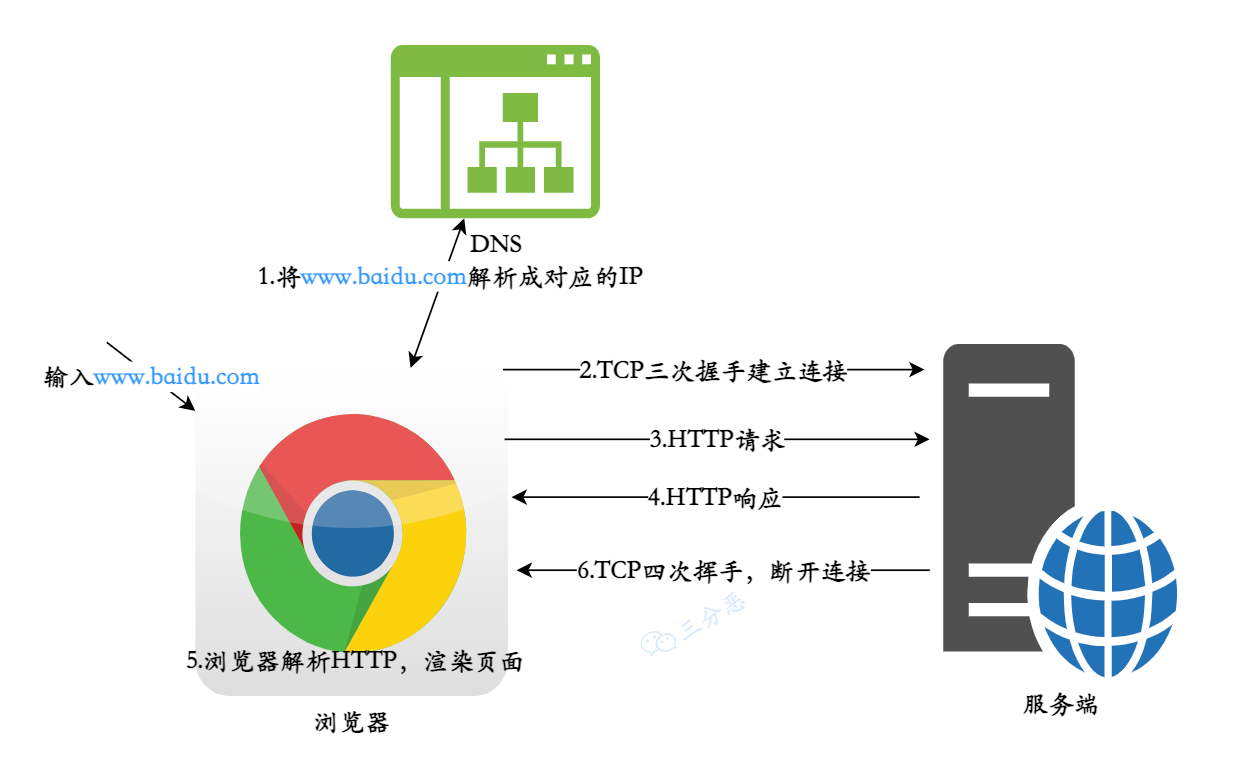
\includegraphics[width=0.95\textwidth]{./Chapter1/q1_1.png}
\caption{浏览器地址输入到显式主页的过程}
\label{fig1_1}
\end{figure}

各个过程使用到的协议如下图\ref{fig1_2} 所示:
\begin{figure}[htbp]
\centering
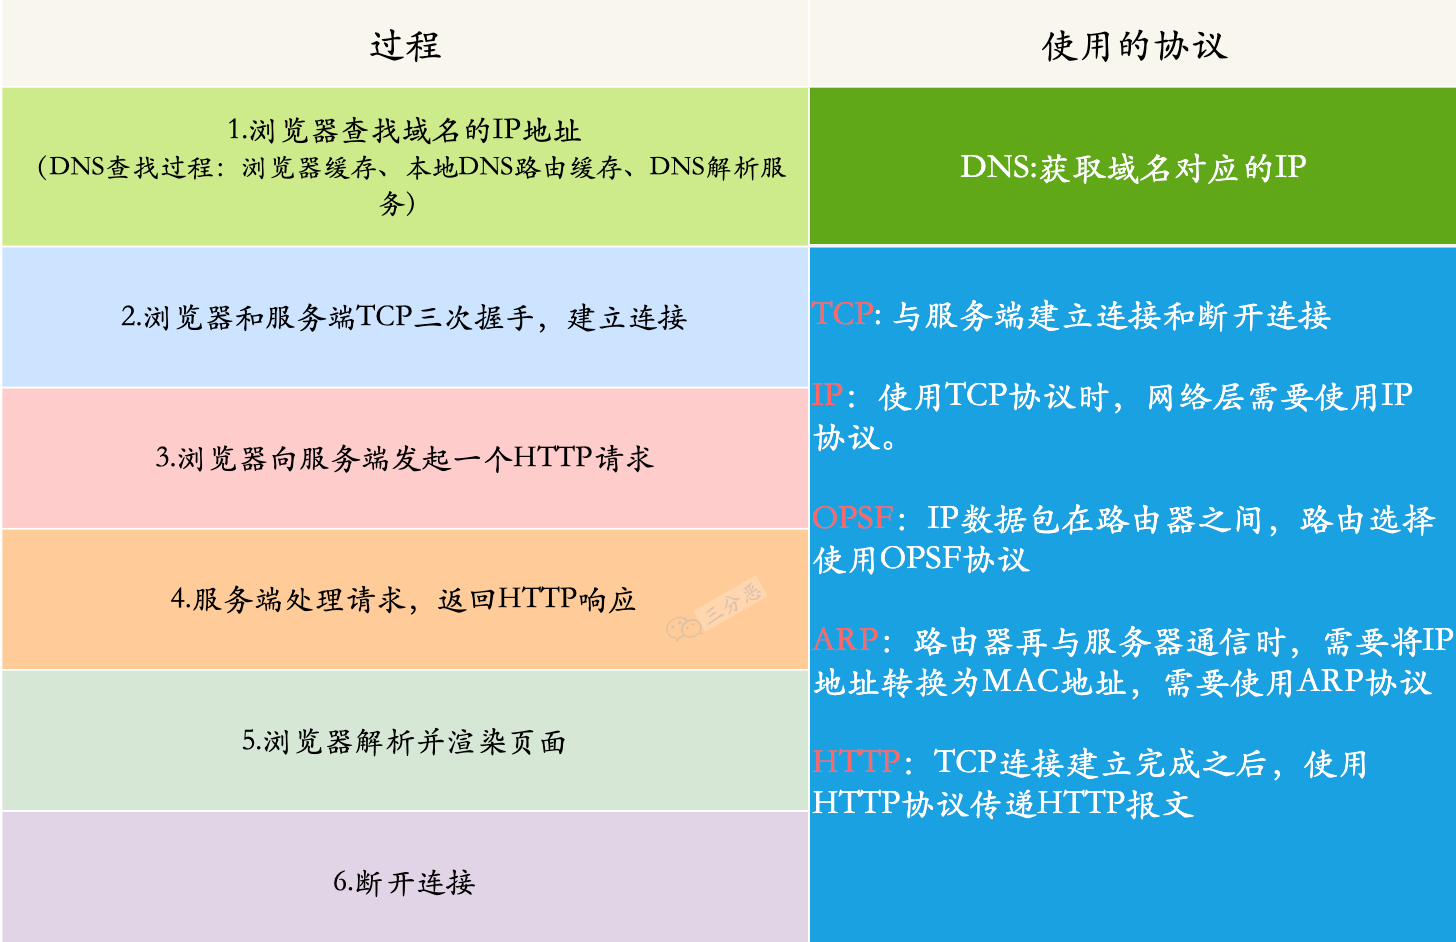
\includegraphics[width=0.95\textwidth]{./Chapter1/q1_2.png}
\caption{每个过程涉及到的协议}
\label{fig1_2}
\end{figure}
\end{solution}

% ----------------------- 问题2 ----------------------
\begin{custom}{问题2}
输入网址到渲染界面过程?
\end{custom}
\begin{solution}
发送http请求--->看本地缓存--->DNS解析出域名对应的IP地址--->TCP/IP五层协议--->可能会有代理(正向代理反向代理)--->TCP连接三次握手 / https认证,加密,解密--->找到端口号--->nignx反向代理将请求分发到具体服务器主机--->mvc框架下从views找到路由--->验证权限--->解析url参数--->看服务器中的缓存--->代码逻辑中获取数据并返回html模板--->服务端发送http响应--->浏览器渲染页面
\end{solution}

% ----------------------- 问题3 ---------------------
\begin{custom}{问题3}
正向代理和反向代理区别?
\end{custom}
\begin{solution}
首先代理是指:客户端主机借助代理服务器访问目标服务器。
\begin{itemize}
\item 客户端 -request-> 代理 -request-> 服务器
\item 客户端 <-response- 代理 <-response- 服务器
\end{itemize}

正向代理:客户端借助代理访问无法访问的服务器,客户端需要配置。

反向代理:服务端借助代理实现负载均衡,客户端无需配置,也不知道自己经过了代理。
\end{solution}

% ------------------ 问题4 ------------------------
\begin{custom}{问题4}
说一下你了解的端口及对应的服务
\end{custom}
\begin{solution}
常用的端口和作用如下图\ref{fig4_1} 所示:
\begin{figure}[htbp]
\centering
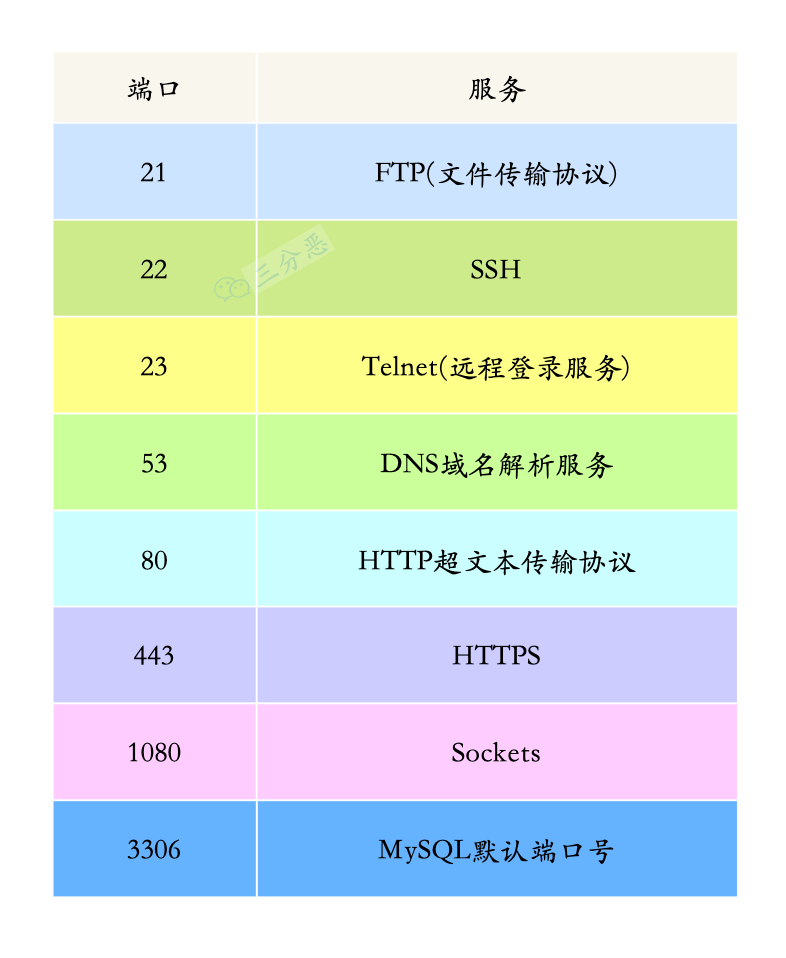
\includegraphics[width=0.95\textwidth]{./Chapter1/q4_1.png}
\caption{常见端口及对应服务}
\label{fig4_1}
\end{figure}

\end{solution}

% ---------------------- 问题5 ----------------
\begin{custom}{问题5}
介绍一下CDN?
\end{custom}
\begin{solution}
视频讲解链接:\href{https://www.zhihu.com/zvideo/1338850254489939968}{https://www.zhihu.com/zvideo/1338850254489939968},后续需要文字整理一下。
\end{solution}

% --- 问题6 ---
\begin{custom}{问题6}
cookie跨域
\end{custom}
\begin{solution}
目前还没有写答案,需要更新
\end{solution}

\chapter{计算机网络体系}
% ------------- 问题 7 --------------
\begin{custom}{问题7}
说下计算机网络体系结构
\end{custom}
\begin{solution}
计算机网络体系结构,一般有 3 种:OSI 七层模型、五层结构、TCP/IP 四层模型,如下图\ref{fig7_1} 所示:

\begin{figure}[htbp]
\centering
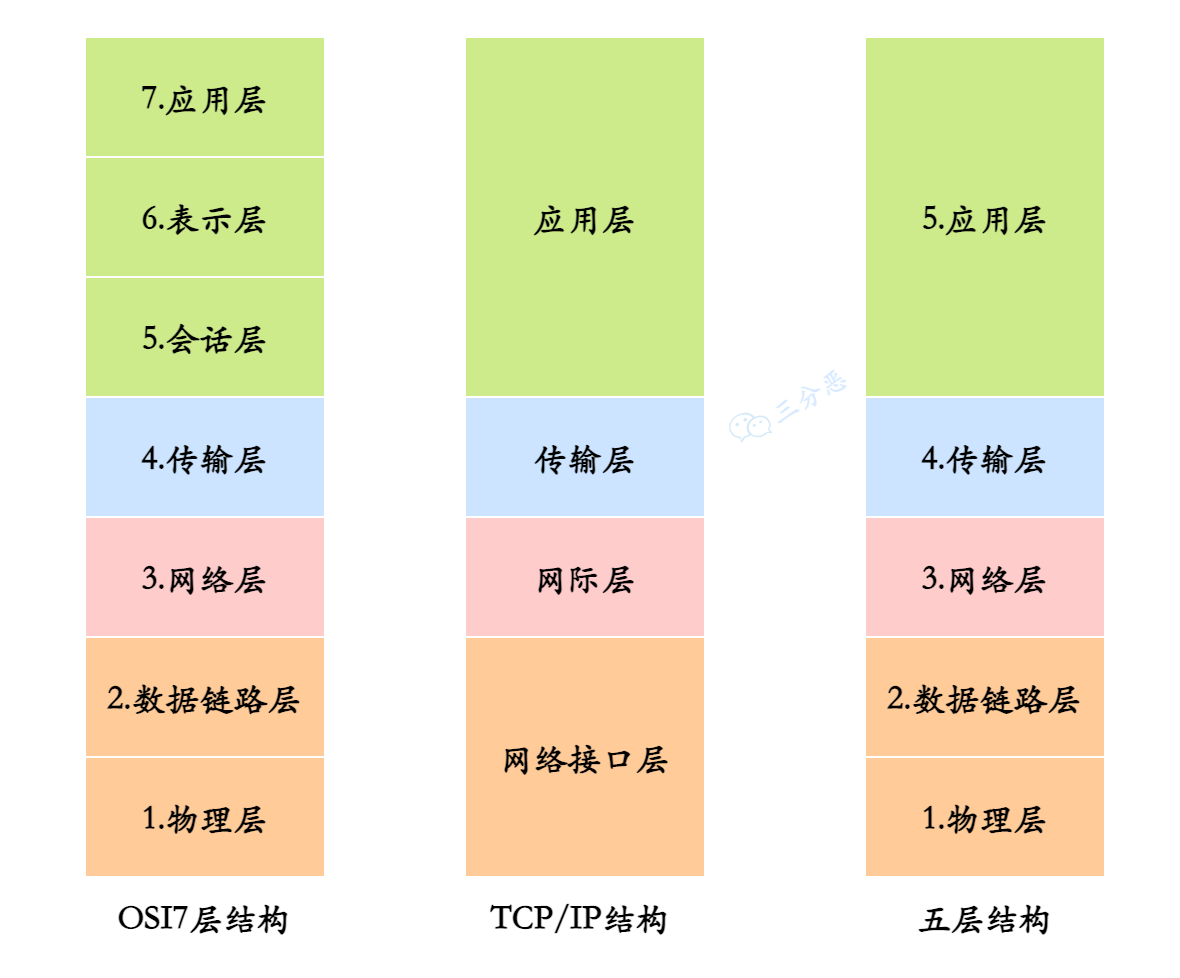
\includegraphics[width=0.95\textwidth]{./Chapter2/q7_1.png}
\caption{3 种计算机网络体系}
\label{fig7_1}
\end{figure}
简单说,OSI 是一个理论上的网络通信模型,TCP/IP 是实际上的网络通信模型,五层结构就是为了介绍网络原理而折中的网络通信模型。

\begin{note} \textbf{OSI 七层模型} \end{note}

OSI 七层模型是国际标准化组织(International Organization for Standardization)制定的一个用于计算机或通信系统间互联的标准体系。
\begin{enumerate}
\item 应用层:通过应用进程之间的交互来完成特定网络应用,应用层协议定义的是应用进程间通信和交互的规则,常见的协议有:HTTP FTP SMTP SNMP DNS.
\item 表示层:数据的表示、安全、压缩。确保一个系统的应用层所发送的信息可以被另一个系统的应用层读取。
\item 会话层:建立、管理、终止会话,是用户应用程序和网络之间的接口。
\item 运输层:提供源端与目的端之间提供可靠的透明数据传输,传输层协议为不同主机上运行的进程提供逻辑通信。
\item 网络层:将网络地址翻译成对应的物理地址,实现不同网络之间的路径选择, 协议有 ICMP, IGMP, IP 等。
\item 数据链路层:在物理层提供比特流服务的基础上,建立相邻结点之间的数据链路。
\item 物理层:建立、维护、断开物理连接。
\end{enumerate}

\begin{note} \textbf{五层体系结构} \end{note}
\begin{enumerate}
\item 应用层:对应于 OSI 参考模型的(应用层、表示层、会话层)。
\item 传输层:对应 OSI 参考模型的的传输层。
\item 网络层:对应 OSI 参考模型的的网络层。
\item 数据链路层:对应 OSI 参考模型的的数据链路层。
\item 物理层:对应 OSI 参考模型的的物理层。
\end{enumerate}

\begin{note} \textbf{TCP/IP 四层结构} \end{note}
\begin{enumerate}
\item 应用层:对应于 OSI 参考模型的(应用层、表示层、会话层)。
\item 传输层: 对应 OSI 的传输层,为应用层实体提供端到端的通信功能,保证了数据包的顺序传送及数据的完整性。
\item 网际层:对应于 OSI 参考模型的网络层,主要解决主机到主机的通信问题。
\item 网络接口层:与 OSI 参考模型的数据链路层、物理层对应。
\end{enumerate}
\end{solution}

% ----------------------- 问题8 ---------------------
\begin{custom}{问题8}
说一下每一层对应的网络协议有哪些?
\end{custom}
\begin{solution}
一张表格总结常见网络协议,如下图\ref{fig8_1} 所示:

\begin{figure}[htbp]
\centering
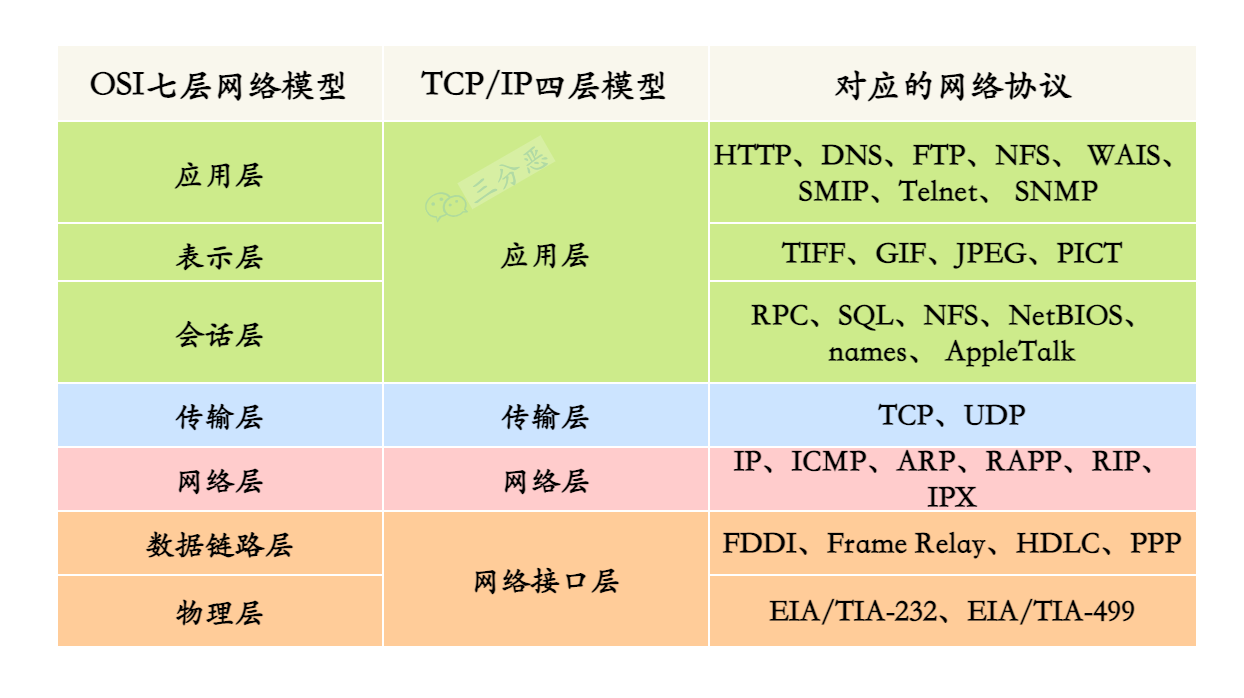
\includegraphics[width=0.95\textwidth]{./Chapter2/q8_1.png}
\caption{计算机网络体系每层对应网络协议}
\label{fig8_1}
\end{figure}
\end{solution}

% -------------------- 问题9 --------------------
\begin{custom}{问题9}
数据在各层之间是怎么传输的呢?
\end{custom}
\begin{solution}
对于发送方而言,从上层到下层层层包装;对于接收方而言,从下层到上层,层层解开包装。
\begin{enumerate}
\item 发送方的\textbf{应用进程}(如 QQ 等某个应用程序)向接收方的应用进程传送数据;
\item AP (application) 先将数据交给本主机的\textbf{应用层},应用层加上本层的控制信息 H5 就变成了下一层的数据单元;
\item \textbf{传输层}收到这个数据单元后,加上本层的控制信息 H4,再交给网络层,成为网络层的数据单元;
\item 到了\textbf{数据链路层},控制信息被分成两部分,分别加到本层数据单元的首部(H2)和尾部(T2);
\item 最后的\textbf{物理层},进行比特流的传输
\end{enumerate}
\end{solution}

上述过程如下图\ref{fig9_1} 所示,这个过程类似写信,写一封信,每到一层,就加一个信封,写一些地址的信息。到了目的地之后,又一层层解封,传向下一个目的地。
\begin{figure}[htbp]
\centering
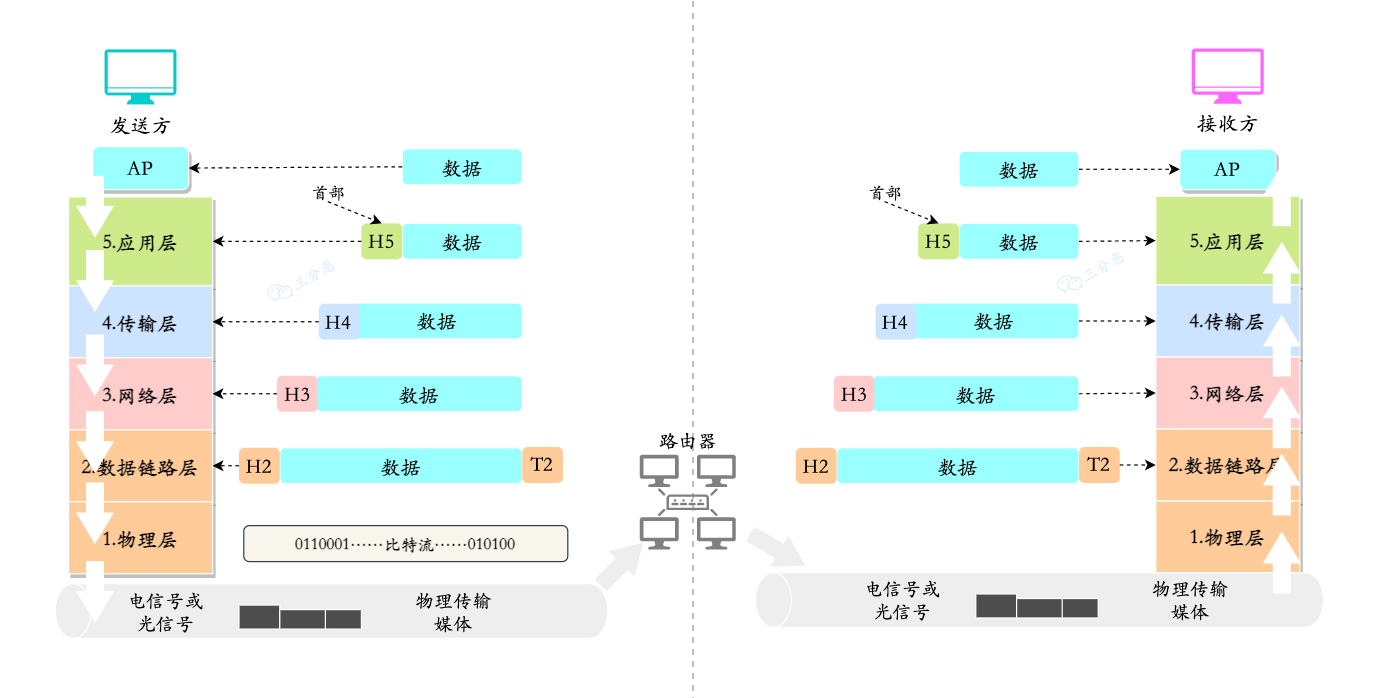
\includegraphics[width=1.0\textwidth]{./Chapter2/q9_1.png}
\caption{计算机网络体系每层对应网络协议}
\label{fig9_1}
\end{figure}

\chapter{应用层对应问题}

% --------------- 问题10 ---------------------
\begin{custom}{问题10}
DNS解析原理和过程?
\end{custom}
\begin{solution}
\begin{note} \textbf{DNS 解析过程} \end{note}
DNS,英文全称是 domain name system,域名解析系统,它的作用也很明确,就是域名和 IP 相互映射。

DNS 的解析过程如下图\ref{fig10_1} 所示:

\begin{figure}[htbp]
\centering
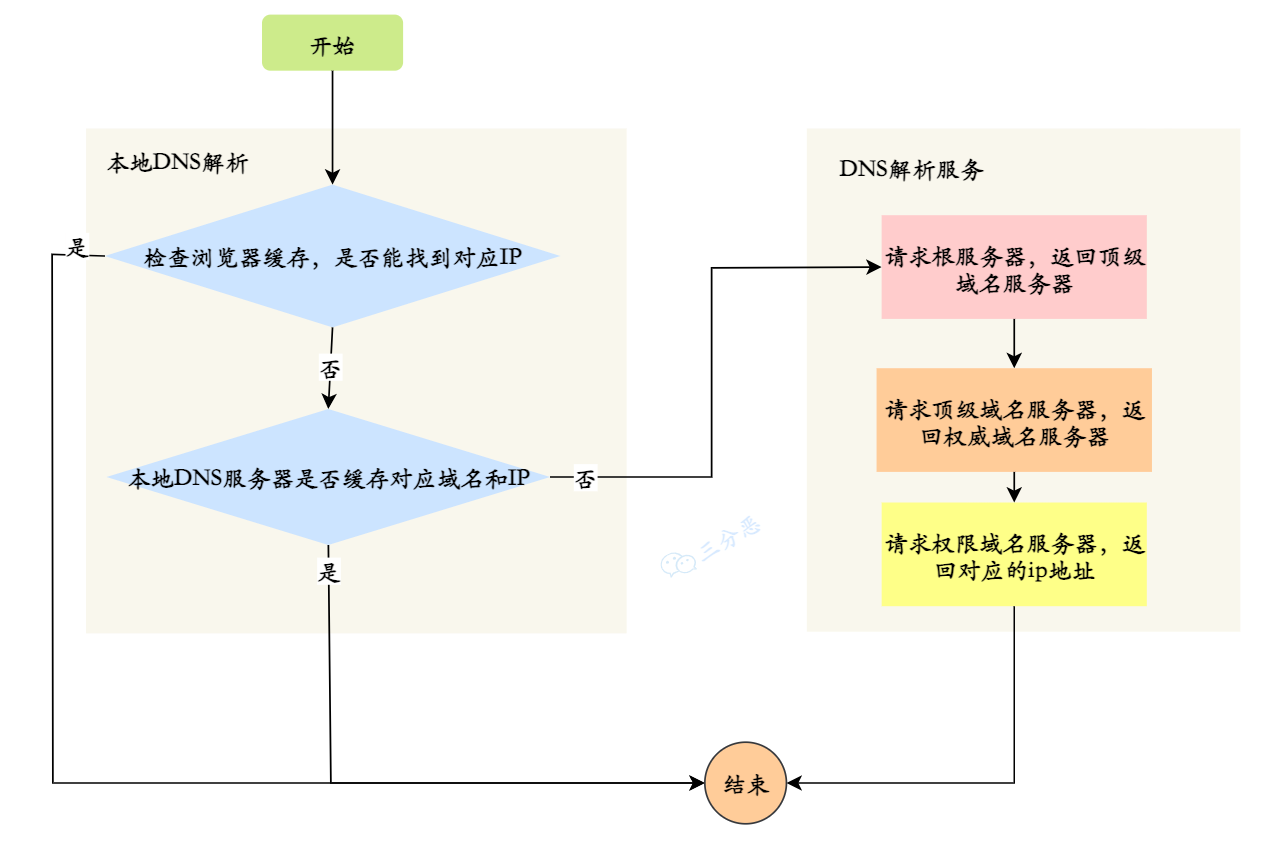
\includegraphics[width=1.0\textwidth]{./Chapter3/q10_1.png}
\caption{计算机网络体系每层对应网络协议}
\label{fig10_1}
\end{figure}

假设你要查询 www.baidu.com 的 IP 地址:
\begin{enumerate}
	\item 首先会查找\textbf{浏览器的缓存},看看是否能找到 www.baidu.com 对应的 IP 地址,找到就直接返回;否则进行下一步。
	\item 将请求发往给\textbf{本地 DNS 服务器},如果查找到也直接返回,否则继续进行下一步;
	\item 本地 DNS 服务器向\textbf{根域名服务器}发送请求,根域名服务器返回负责 com 的顶级域名服务器的 IP 地址的列表。
	\item 本地 DNS 服务器再向其中一个\textbf{负责 com 的顶级域名服务器}发送一个请求,返回负责 baidu.com 的权限域名服务器的 IP 地址列表。
	\item 本地 DNS 服务器再向其中一个\textbf{权限域名服务器}发送一个请求,返回 www.baidu.com 所对应的IP地址
\end{enumerate}

上面提到了本地递归式地查询了:权限域名服务器 --> 顶级域名服务器 --> 根域名服务器,它们的关系如下图\ref{fig10_2} 所示:
\begin{figure}[htbp]
\centering
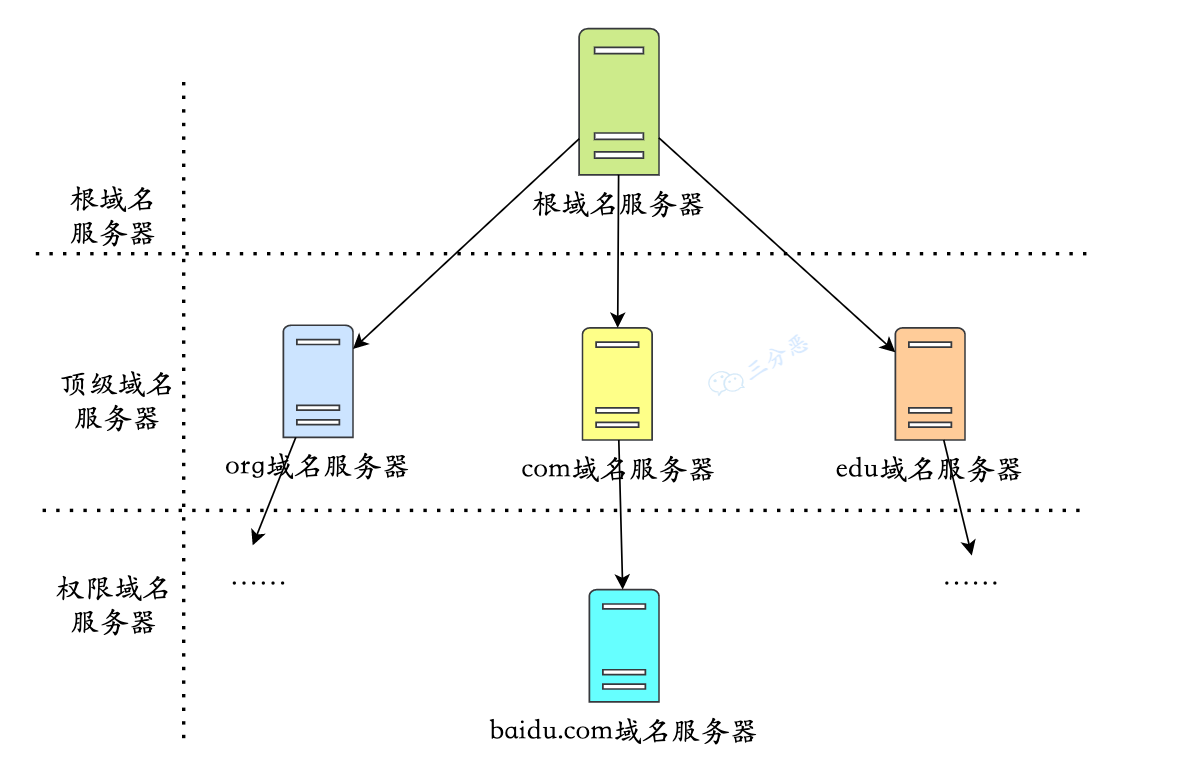
\includegraphics[width=1.0\textwidth]{./Chapter3/q10_2.png}
\caption{计算机网络体系每层对应网络协议}
\label{fig10_2}
\end{figure}

另外,对上面的本地 DNS 服务器和权威服务器做一个概念上的补充,如下所示:
\begin{myDefinition}{本地 DNS 服务器}{example}

本地 DNS 一般是指你电脑上网时 IPv4 或者 IPv6 设置中填写的那个 DNS,这个有可能是手工指定的或者是 DHCP 自动分配的。如果你的电脑是直连运营商网络,一般默认设置情况下 DNS 为 DHCP 分配到的运营商的服务器地址。

如果你的电脑和运营商之间还加了无线或者有线路由,那极有可能路由器本身还内置了一个 DNS 转发器,这玩意的作用是将发往他所有的 DNS 请求转发到上层 DNS。此时由于路由器本身也接管了下挂电脑的 DHCP 服务,所以它分配给下面电脑的 DNS 地址就是它自身,所以你能看到电脑的 DNS 分配到的可能是 192.168.1.1。实际上就是路由器自身,而路由器的 DNS 转发器将请求转发到上层 ISP 的 DNS。所以这里说 DNS 是局域网或者是运营商的都可以(因为最终都是转发到运营商,小细节不用纠结)。
\end{myDefinition}

\begin{myDefinition}{权威服务器}{example}
权威服务器是特殊的DNS服务器,所谓的权威是针对特定域名来说的。所以一般会说某某域名的权威DNS是谁,不能单纯的抛离域名问权威DNS是谁。是域名商在管理,负责解析在他这里购买的域名的权威解析(当然也存在此处购买域名挂靠别处权威的情况。同样,不要纠结于小细节,意思懂了就行。如果要了解原理请查找一下NS记录这个名词)。
\end{myDefinition}

\begin{note} \textbf{DNS 解析原理} \end{note}
上面已经详细说明了解析的步骤,下面是上述每一步涉及到的理论:
\begin{enumerate} 
	\item 浏览器输入域名, 操作系统\textbf{检查自己本地的 hosts 文件是否有这个网址映射关系},如果有,就先调度这个 IP 地址映射,完成域名解析;如果没有,则\textbf{查找本地 DNS 解析器缓存}。
	\item 如果还没有,则\textbf{找到 TCP/IP 参数中设置的首选 DNS 服务器},DNS 服务器查询域名(具有权威性);如果此域名不由 DNS 服务器区域解析,但该服务器缓存了网址映射关系(则没有权威性)。
	\item 如果查询都失效,则\textbf{查看本地 DNS 服务器是否开转发模式,如未开,则把请求发至根服务器。}根服务器判断这个域名谁授权管理,并返回一个负责该顶级域名服务器的IP。
	\item 本地 DNS 服务器收到 IP 信息后,将会联系负责 .com 域的这台服务器。如果这台服务器无法解析,就会找到下一级 DNS 服务器地址 (http://qq.com) 给本地 DNS 服务器。重复以上操作,直到找到http://www.qq.com 主机。
	\item 如果是转发模式,此 DNS 服务器就会把请求转发至上一级 DNS 服务器,上一级服务器进行解析。如果不行,就上上级,以此循环。
\end{enumerate}
\end{solution}

%--------------- 问题11 -------------------
\begin{custom}{问题11}
说说 WebSocket 与 Socket 的区别
\end{custom}
\begin{solution}
Socket 一个是网编编程的标准接口,而 WebSocket 则是应用层通信协议。

\begin{itemize}
	\item Socket 其实就是等于:IP 地址 + 端口 + 协议。具体来说,Socket 是一套标准,它完成了对 TCP/IP 的高度封装,屏蔽网络细节,以方便开发者更好地进行网络编程。
	\item WebSocket 是一个持久化的协议,它是伴随 H5 而出的协议,用来解决 http 不支持持久化连接的问题
\end{itemize}

\end{solution}

%------------- 问题12 -----------------
\begin{custom}{问题12}
HTTP 请求的过程与原理?
\end{custom}

\begin{solution}
HTTP 协议定义了浏览器怎么向服务器请求文档,以及服务器怎么把文档传给浏览器。HTTP 请求过程如下图\ref{fig12_1} 所示
\begin{figure}[!h]
\centering
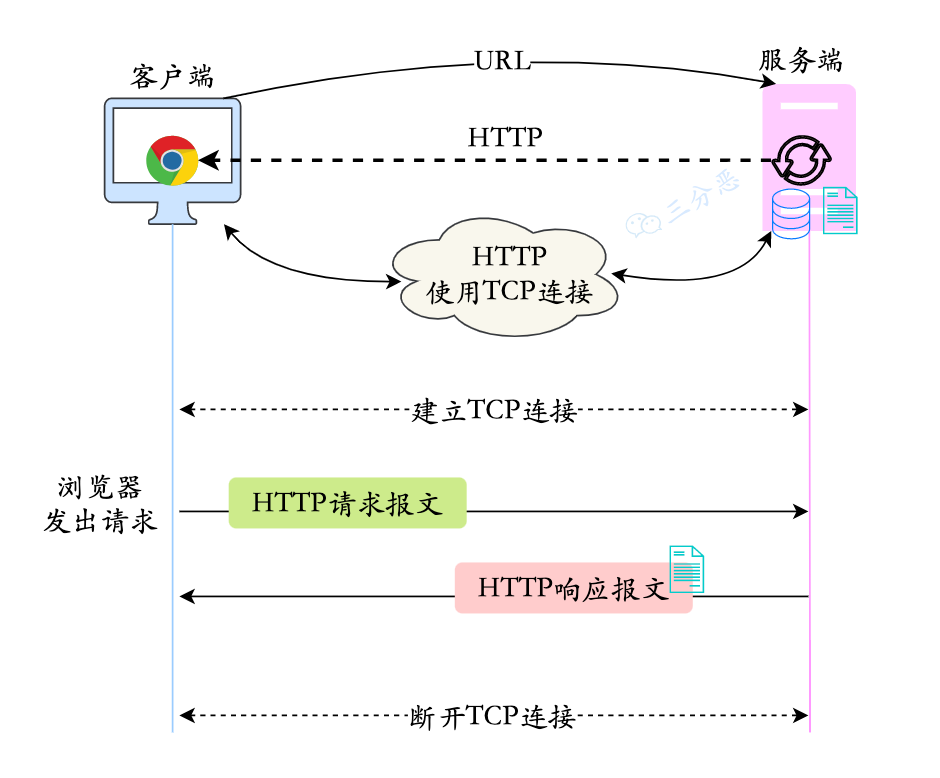
\includegraphics[width=0.6\textwidth]{./Chapter3/q12_1.png}
\caption{HTTP 请求过程}
\label{fig12_1}
\end{figure}

在这个过程中:
\begin{itemize}
	\item 每个服务器都有一个进程,它不断监听 TCP 的端口 80,以便发现是否有浏览器向它发出连接建立请求;
	\item 监听到连接请求,就会建立 TCP 连接;
	\item 浏览器向服务器发出浏览某个页面的请求,服务器接着就返回所请求的页面作为响应;
	\item 最后,释放 TCP 连接。
\end{itemize}
在浏览器和服务器之间的请求和响应的交互,必须按照规定的格式和遵循一定的规则,这些格式和规则就是超文本传输协议 HTTP。 PS:这道题和上面浏览器输入网址发生了什么那道题大差不差。
\end{solution}

%---------- 问题14 ---------------
\begin{custom}{问题14}
说说 HTTP 常用的状态码及其含义?
\end{custom}
\begin{solution}
\href{https://www.runoob.com/http/http-status-codes.html}{HTTP状态码}首先应该知道个大概的分类:
\begin{itemize}
	\item 1XX:信息性状态码
	\item 2XX:成功状态码
	\item 3XX:重定向状态码
	\item 4XX:客户端错误状态码
	\item 5XX:服务端错误状态码
\end{itemize}
几个常用的状态码如下图\ref{fig14_1} 所示,也应该记住:
\begin{figure}[htbp]
\centering
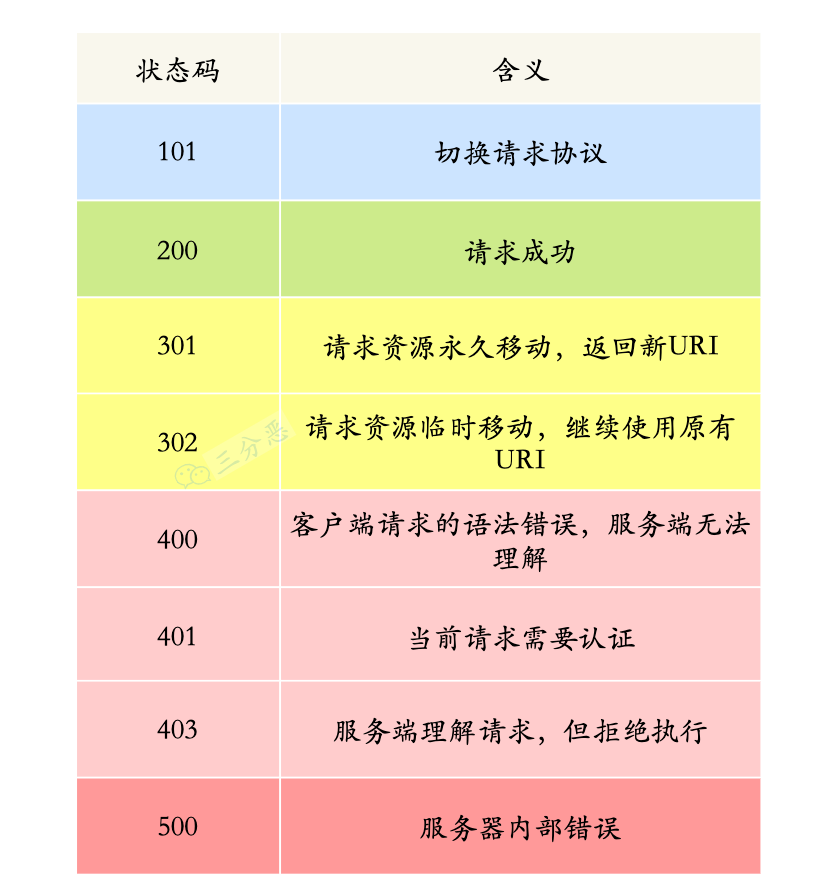
\includegraphics[width=0.7\textwidth]{./Chapter3/q14_1.png}
\caption{常见的状态码}
\label{fig14_1}
\end{figure}
\end{solution}

%---------------- 问题15 ----------------
\begin{custom}{问题15}
说一下HTTP的报文结构?
\end{custom}

\begin{solution}
HTTP 报文有两种,HTTP 请求报文和 HTTP 响应报文,大致结构如下图\ref{fig15_1} 所示:
\begin{figure}[htbp]
\centering
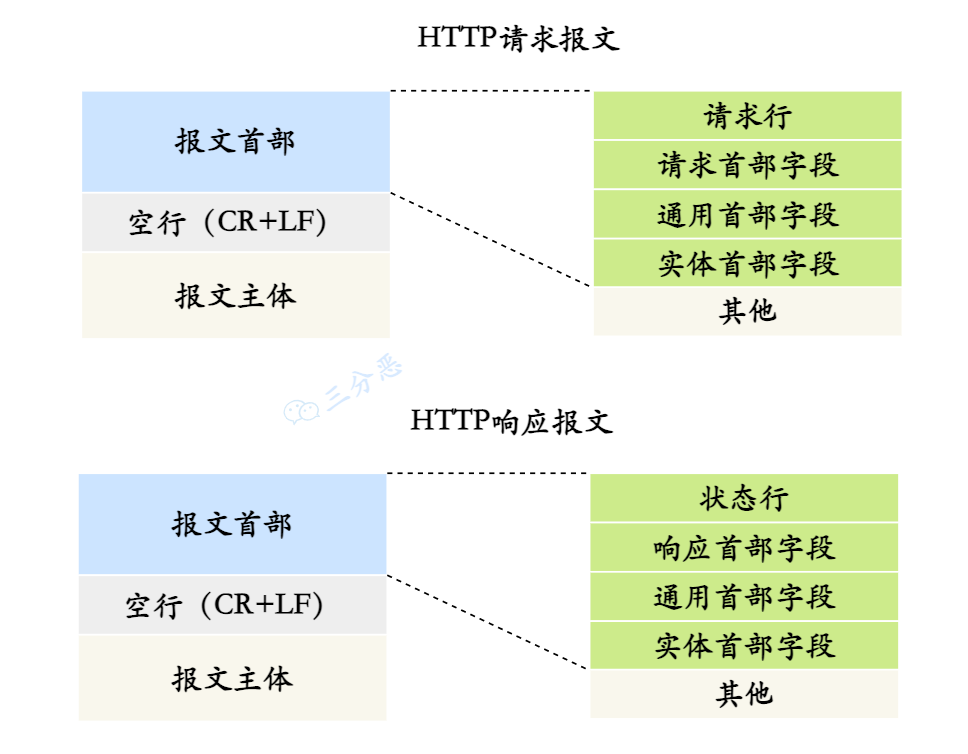
\includegraphics[width=0.7\textwidth]{./Chapter3/q15_1.png}
\caption{HTTP 请求报文和响应报文的大致结构}
\label{fig15_1}
\end{figure}

\begin{note} \textbf{HTTP 请求报文} \end{note}
HTTP 请求报文的格式如下:

\begin{lstlisting}
GET / HTTP/1.1                                                   
User-Agent: Mozilla/5.0 (Macintosh; Intel Mac OS X 10_10_5)      
Accept: */*                                                       
\end{lstlisting}

HTTP 请求报文的第一行叫做请求行,后面的行叫做首部行,首部行后还可以跟一个实体主体。请求首部之后有一个空行,这个空行不能省略,它用来划分首部与实体。

请求行包含三个字段:
\begin{itemize}
	\item 方法字段:包括 POST、GET 等请方法。
	\item URL 字段
	\item HTTP 版本字段。
\end{itemize}

\begin{note} \textbf{响应报文} \end{note}
HTTP 响应报文的格式如下:
\begin{lstlisting}
HTTP/1.0 200 OK                                    

Content-Type: text/plain
Content-Length: 137582                             
Expires: Thu, 05 Dec 1997 16:00:00 GMT             
Last-Modified: Wed, 5 August 1996 15:55:28 GMT     
Server: Apache 0.84
<html>
  <body>Hello World</body>
</html>                                                     
\end{lstlisting}

\begin{itemize}
	\item 状态行包含了三个字段:协议版本字段、状态码和相应的状态信息。
	\item 首部行首部可以分为四种首部,请求首部、响应首部、通用首部和实体首部。通用首部和实体首部在请求报文和响应报文中都可以设置,区别在于请求首部和响应首部。
	\begin{itemize}
		\item 常见的请求首部有 Accept 可接收媒体资源的类型、Accept-Charset 可接收的字符集、Host 请求的主机名。
		\item 常见的响应首部有 ETag 资源的匹配信息,Location 客户端重定向的 URI。
		\item 常见的通用首部有 Cache-Control 控制缓存策略、Connection 管理持久连接。
		\item 常见的实体首部有 Content-Length 实体主体的大小、Expires 实体主体的过期时间、Last-Modified 资源的最后修改时间。
	\end{itemize}
	\item 实体部分是报文的主要部分,它包含了所请求的对象。
\end{itemize}
\end{solution}

% ------------- 问题16 --------------
\begin{custom}{问题16}
URI 和 URL 有什么区别?
\end{custom}

\begin{solution}
URI 是 URL 的一个子集,如下图\ref{fig16_1} 所示:
\begin{figure}[htbp]
\centering
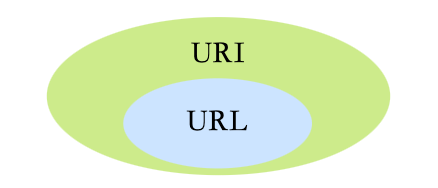
\includegraphics[width=0.6\textwidth]{./Chapter3/q16_1.png}
\caption{URI 和 URL 关系}
\label{fig16_1}
\end{figure}

它们的主要区别在于,URL 除了提供了资源的标识,还提供了资源访问的方式。这么比喻,URI 像是身份证,可以唯一标识一个人;而 URL 更像一个住址,可以通过 URL 找到这个人——人类住址协议://地球/中国/北京市/海淀区/xx职业技术学院/14号宿舍楼/525号寝/张三.男。
\begin{itemize}
	\item URI,统一资源标识符(Uniform Resource Identifier, URI),标识的是 Web 上每一种可用的资源,如 HTML 文档、图像、视频片段、程序等都是由一个 URI 进行标识的。
	\item URL,统一资源定位符(Uniform Resource Location),它是 URI 的一种子集,主要作用是提供资源的路径。
\end{itemize}
\end{solution}

%------------- 问题17 ---------------
\begin{custom}{问题17}
HTTP 有哪些请求方式?
\end{custom}
\begin{solution}
这里的请求方式是指报文的类型,如下图\ref{fig17_1} 所示:
\begin{figure}[!h]
\centering
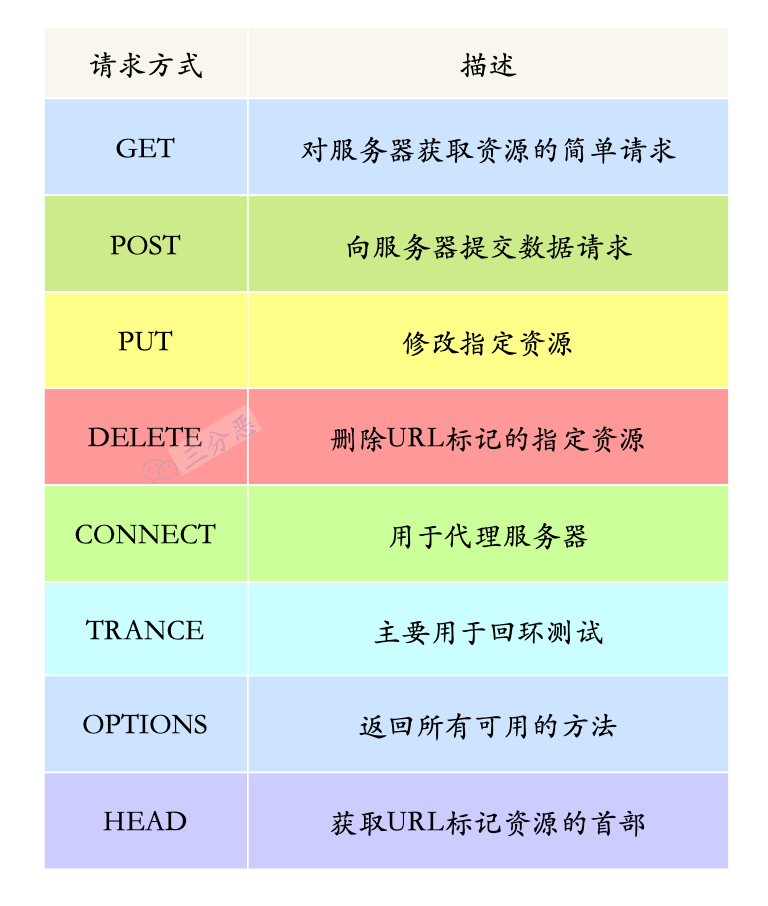
\includegraphics[width=0.7\textwidth]{./Chapter3/q17_1.png}
\caption{各种请求关键字}
\label{fig17_1}
\end{figure}
其中,POST、DELETE、PUT、GET的含义分别对应我们最熟悉的增、删、改、查。
\end{solution}
\newpage
%------------ 问题18 ------------------
\begin{custom}{问题18}
说⼀下 GET 和 POST 的区别?
\end{custom}
\begin{solution}
可以从以下几个方面来说明 GET 和 POST 的区别,如下图\ref{fig18_1} 所示:
\begin{figure}[htbp]
\centering
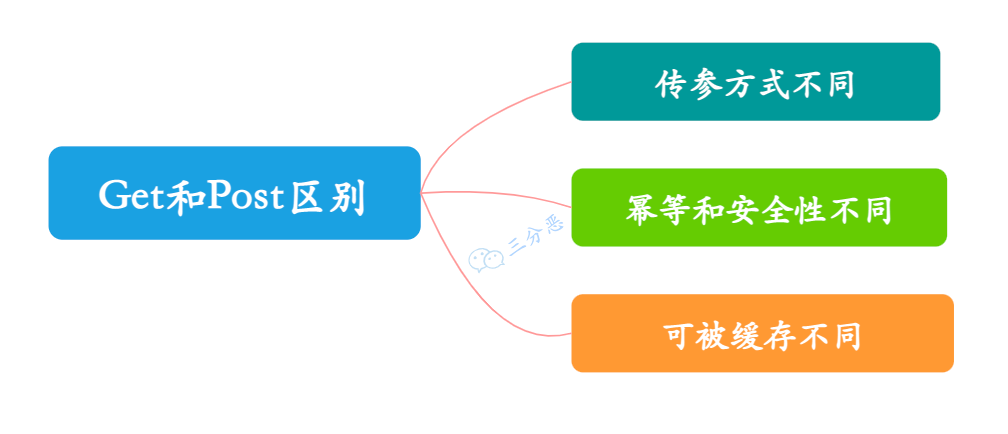
\includegraphics[width=0.7\textwidth]{./Chapter3/q18_1.png}
\caption{GET 和 POST 区别}
\label{fig18_1}
\end{figure}
具体来说
\begin{itemize}
	\item 从 HTTP 报文层面来看,GET 请求将信息放在 URL,POST 将请求信息放在请求体中。这一点使得 GET 请求携带的数据量有限,因为 URL 本身是有长度限制的,而 POST 请求的数据存放在报文体中,因此对大小没有限制。而且从形式上看,GET 请求把数据放 URL 上不太安全,而 POST 请求把数据放在请求体里想比较而言安全一些。
	\item 从数据库层面来看,GET 符合幂等性和安全性,而 POST 请求不符合。这个其实和 GET/POST 请求的作用有关。按照 HTTP 的约定,GET 请求用于查看信息,不会改变服务器上的信息;而 POST 请求用来改变服务器上的信息。正因为 GET 请求只查看信息,不改变信息,对数据库的一次或多次操作获得的结果是一致的,认为它符合幂等性。安全性是指对数据库操作没有改变数据库中的数据。
	\item 从其他层面来看,GET 请求能够被缓存,GET 请求能够保存在浏览器的浏览记录里,GET 请求的 URL 能够保存为浏览器书签。这些都是 POST 请求所不具备的。缓存是 GET 请求被广泛应用的根本,他能够被缓存也是因为它的幂等性和安全性,除了返回结果没有其他多余的动作,因此绝大部分的 GET 请求都被 CDN 缓存起来了,大大减少了 Web 服务器的负担。
\end{itemize}

\end{solution}

% --------- 问题19 --------------
\begin{custom}{问题19}
PUT和POST有什么区别?
\end{custom}
\begin{solution}
xxxxxxxxxxxxxxxxxxxxxx
\end{solution}

% --------- 问题20 --------------
\begin{custom}{问题20}
GET 的长度限制是多少?
\end{custom}
\begin{solution}
HTTP 中的 GET 方法是通过 URL 传递数据的,但是 URL 本身其实并没有对数据的长度进行限制,真正限制 GET 长度的是浏览器。

例如 IE 浏览器对 URL 的最大限制是 2000 多个字符,大概 2kb 左右,像 Chrome、Firefox 等浏览器支持的 URL 字符数更多,其中 FireFox 中 URL 的最大长度限制是 65536 个字符,Chrome 则是 8182个字符。

这个长度限制也不是针对数据部分,而是针对整个 URL。
\end{solution}

% --------- 问题21 --------------
\begin{custom}{问题21}
说下 HTTP/1.0,1.1,2.0 的区别
\end{custom}
\begin{solution}
关键需要记住 HTTP/1.0 默认是短连接,可以强制开启,HTTP/1.1 默认长连接,HTTP/2.0 采用多路复用。
\begin{note} \textbf{HTTP/1.0} \end{note}
默认使用短连接,每次请求都需要建立一个 TCP 连接。它可以设置Connection: keep-alive 这个字段,强制开启长连接。

\begin{note} \textbf{HTTP/1.1} \end{note}
\begin{itemize}
	\item 引入了持久连接,即 TCP 连接默认不关闭,可以被多个请求复用。
	\item 分块传输编码,即服务端每产生一块数据,就发送一块,用” 流模式” 取代” 缓存模式”。
	\item 管道机制,即在同一个 TCP 连接里面,客户端可以同时发送多个请求。
\end{itemize}

\begin{note} \textbf{HTTP/2.0} \end{note}
\begin{itemize}
	\item 二进制协议,1.1 版本的头信息是文本(ASCII 编码),数据体可以是文本或者二进制;2.0 中,头信息和数据体都是二进制。
	\item 完全多路复用,在一个连接里,客户端和浏览器都可以同时发送多个请求或回应,而且不用按照顺序一一对应。
	\item 报头压缩,HTTP 协议不带有状态,每次请求都必须附上所有信息。Http/2.0 引入了头信息压缩机制,使用 gzip 或 compress 压缩后再发送。
	\item 服务端推送,允许服务器未经请求,主动向客户端发送资源。
\end{itemize}
\end{solution}

% --------- 问题22 --------------
\begin{custom}{问题22}
HTTP/3了解吗?
\end{custom}
\begin{solution}

HTTP/3 主要有两大变化,\textbf{传输层基于 UDP}、使用 \textbf{QUIC 保证 UDP 可靠性}。

HTTP/2 存在的一些问题,比如重传等等,都是由于 TCP 本身的特性导致的,所以 HTTP/3 在 QUIC 的基础上进行发展而来,QUIC(Quick UDP Connections)直译为快速 UDP 网络连接,底层使用UDP 进行数据传输。

HTTP/3 主要有这些特点:

\begin{itemize}
	\item 使用 UDP 作为传输层进行通信
	\item 在 UDP 的基础上 QUIC 协议保证了 HTTP/3 的安全性,在传输的过程中就完成了 TLS 加密握手
	\item HTTPS 要建⽴⼀个连接,要花费 6 次交互,先是建⽴三次握⼿,然后是 TLS/1.3 的三次握⼿。QUIC 直接把以往的 TCP 和 TLS/1.3 的 6 次交互合并成了 3 次,减少了交互次数。
	\item QUIC 有⾃⼰的⼀套机制可以保证传输的可靠性的。当某个流发⽣丢包时,只会阻塞这个流,其他流不会受到影响。
\end{itemize}

我们拿一张图\ref{fig22_1} 看一下 HTTP 协议的变迁:
\begin{figure}[htbp]
\centering
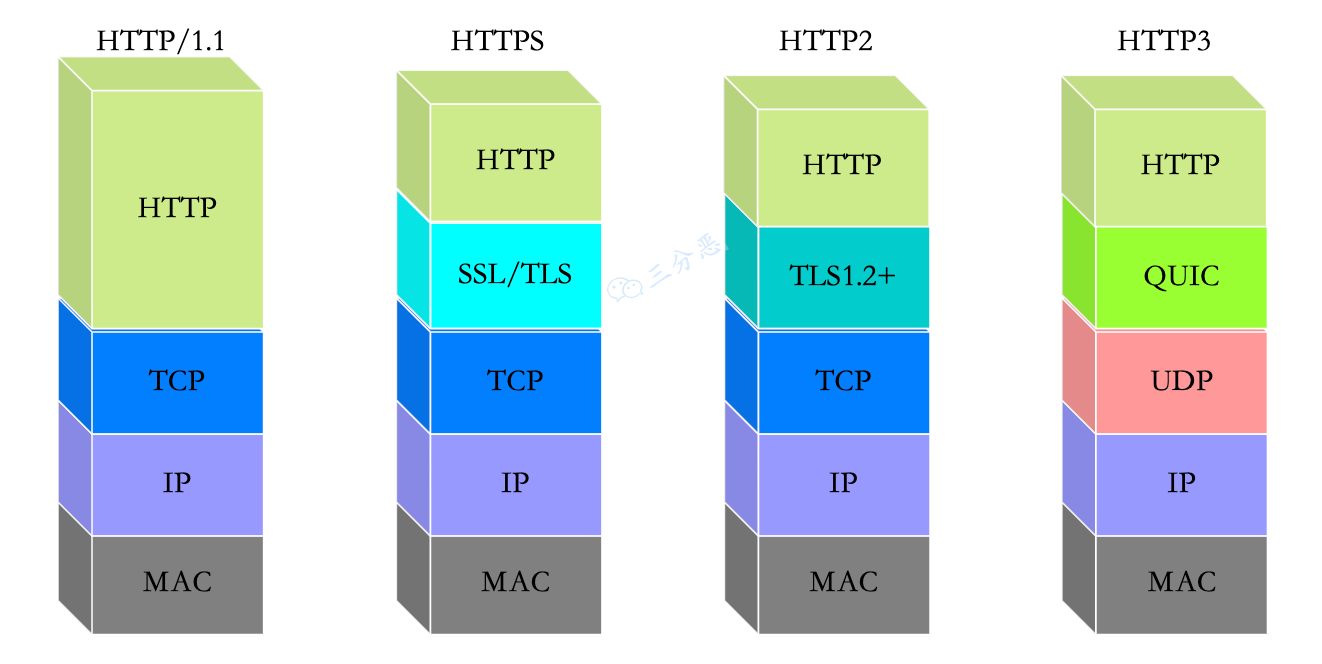
\includegraphics[width=0.7\textwidth]{./Chapter3/q22_1.png}
\caption{HTTP 变迁}
\label{fig22_1}
\end{figure}
\end{solution}

% --------- 问题23 --------------
\begin{custom}{问题19}
HTTP 如何实现长连接?在什么时候会超时?
\end{custom}
\begin{solution}
\begin{note} \textbf{什么是 HTTP 的长连接?} \end{note}

\begin{itemize}
	\item HTTP 分为长连接和短连接,本质上说的是 TCP 的长短连接。TCP 连接是一个双向的通道,它是可以保持一段时间不关闭的,因此 TCP 连接才具有真正的长连接和短连接这一说法。
	\item TCP 长连接可以复用一个 TCP 连接,来发起多次的 HTTP 请求,这样就可以减少资源消耗,比如一次请求 HTML,如果是短连接的话,可能还需要请求后续的 JS/CSS。
\end{itemize}

\begin{note} \textbf{如何设置长连接?} \end{note}
通过在头部(请求和响应头)设置 Connection 字段指定为keep-alive,HTTP/1.0 协议支持,但是是默认关闭的,从 HTTP/1.1 以后,连接默认都是长连接。

\begin{note} \textbf{在什么时候会超时呢?} \end{note}

\begin{itemize}
	\item HTTP 一般会有 httpd 守护进程,里面可以设置 keep-alive timeout,当 tcp 连接闲置超过这个时间就会关闭,也可以在 HTTP 的 header 里面设置超时时间。

	\item TCP 的 keep-alive 包含三个参数,支持在系统内核的 net.ipv4 里面设置;当 TCP 连接之后,闲置了 tcp\_keepalive\_time ,则会发生侦测包,如果没有收到对方的 ACK,那么会每隔 tcp\_keepalive\_intvl 再发一次,直到发送了 tcp\_keepalive\_probes,就会丢弃该连接。
\end{itemize}
\begin{lstlisting}
tcp_keepalive_intvl = 15
tcp_keepalive_probes = 5
tcp_keepalive_time = 1800
\end{lstlisting}

\end{solution}

% --------- 问题24 --------------
\begin{custom}{问题24}
说说HTTP 与 HTTPS 有哪些区别?
\end{custom}
\begin{solution}
\begin{enumerate}
	\item HTTP 是超⽂本传输协议,信息是明⽂传输,存在安全⻛险的问题。HTTPS 则解决 HTTP 不安全的缺陷,在 TCP 和 HTTP ⽹络层之间加⼊了 SSL/TLS 安全协议,使得报⽂能够加密传输。
	\item HTTP 连接建⽴相对简单, TCP 三次握⼿之后便可进⾏ HTTP 的报⽂传输。⽽ HTTPS 在 TCP 三次握⼿之后,还需进⾏ SSL/TLS 的握⼿过程,才可进⼊加密报⽂传输。
	\item HTTP 的端⼝号是 80,HTTPS 的端⼝号是 443。
	\item HTTPS 协议需要向 CA(证书权威机构)申请数字证书,来保证服务器的身份是可信的。
\end{enumerate}
\end{solution}

% --------- 问题25 --------------
\begin{custom}{问题25}
为什么要用HTTPS?解决了哪些问题?
\end{custom}
\begin{solution}
因为 HTTP 是明⽂传输,存在安全上的风险:
\begin{itemize}
	\item 窃听⻛险,⽐如通信链路上可以获取通信内容,用户账号被盗。
	\item 篡改⻛险,⽐如强制植⼊垃圾⼴告,视觉污染。
	\item 冒充⻛险,⽐如冒充淘宝⽹站,用户金钱损失。
\end{itemize}

所以引入了 HTTPS,HTTPS 在 HTTP 与 TCP 层之间加⼊了 SSL/TLS 协议,可以很好的解决了这些风险:
\begin{itemize}
	\item 信息加密:交互信息⽆法被窃取。
	\item 校验机制:⽆法篡改通信内容,篡改了就不能正常显示。
	\item 身份证书:能证明淘宝是真淘宝。
\end{itemize}
所以通过加入下图\ref{fig25_1} 所示的 SSL/TLS 协议,是能保证通信是安全的。
\begin{figure}[htbp]
\centering
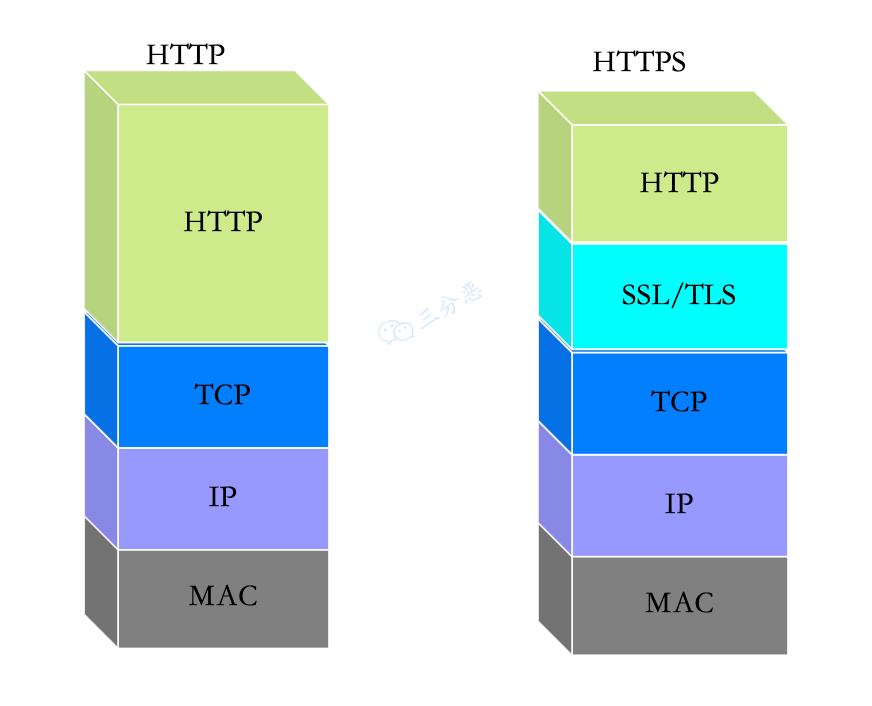
\includegraphics[width=0.7\textwidth]{./Chapter3/q25_1.png}
\caption{SSL/TSL 保证通信安全}
\label{fig25_1}
\end{figure}
\end{solution}

%------------- 问题26 ------------------
\begin{custom}{问题26}
HTTPS工作流程是怎样的?
\end{custom}

\begin{solution}
这道题有几个要点:\textbf{公私钥、数字证书、加密、对称加密、非对称加密}。

HTTPS 主要工作流程:
\begin{enumerate}
	\item 客户端发起 HTTPS 请求,连接到服务端的 443 端口。
	\item 服务端有一套数字证书(证书内容有公钥、证书颁发机构、失效日期等)。
	\item 服务端将自己的数字证书发送给客户端(公钥在证书里面,私钥由服务器持有)。
	\item 客户端收到数字证书之后,会验证证书的合法性。如果证书验证通过,就会生成一个随机的对称密钥,用证书的公钥加密。
	\item 客户端将公钥加密后的密钥发送到服务器。
	\item 服务器接收到客户端发来的密文密钥之后,用自己之前保留的私钥对其进行非对称解密,解密之后就得到客户端的密钥,然后用客户端密钥对返回数据进行对称加密,酱紫传输的数据都是密文啦。
	\item 服务器将加密后的密文返回到客户端。
	\item 客户端收到后,用自己的密钥对其进行对称解密,得到服务器返回的数据。
\end{enumerate}
工作流程如下图\ref{fig26_1} 所示:
\begin{figure}[htbp]
\centering
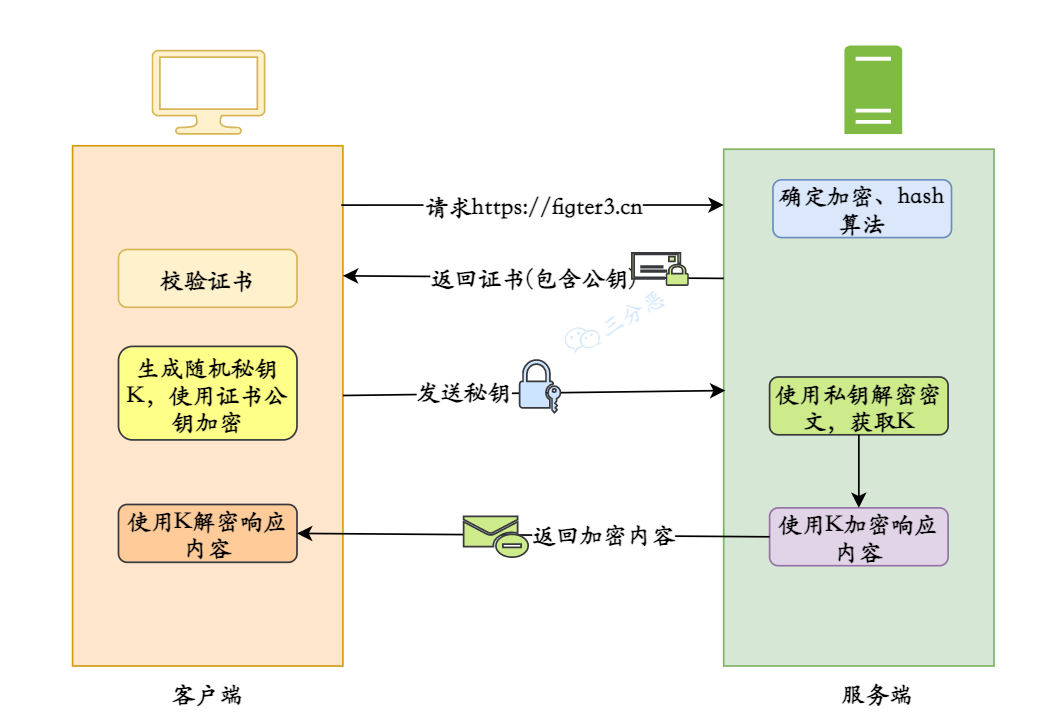
\includegraphics[width=0.7\textwidth]{./Chapter3/q26_1.png}
\caption{HTTPS 主要工作流程}
\label{fig26_1}
\end{figure}

这里还画了一张更详尽的图:
\begin{figure}[htbp]
\centering
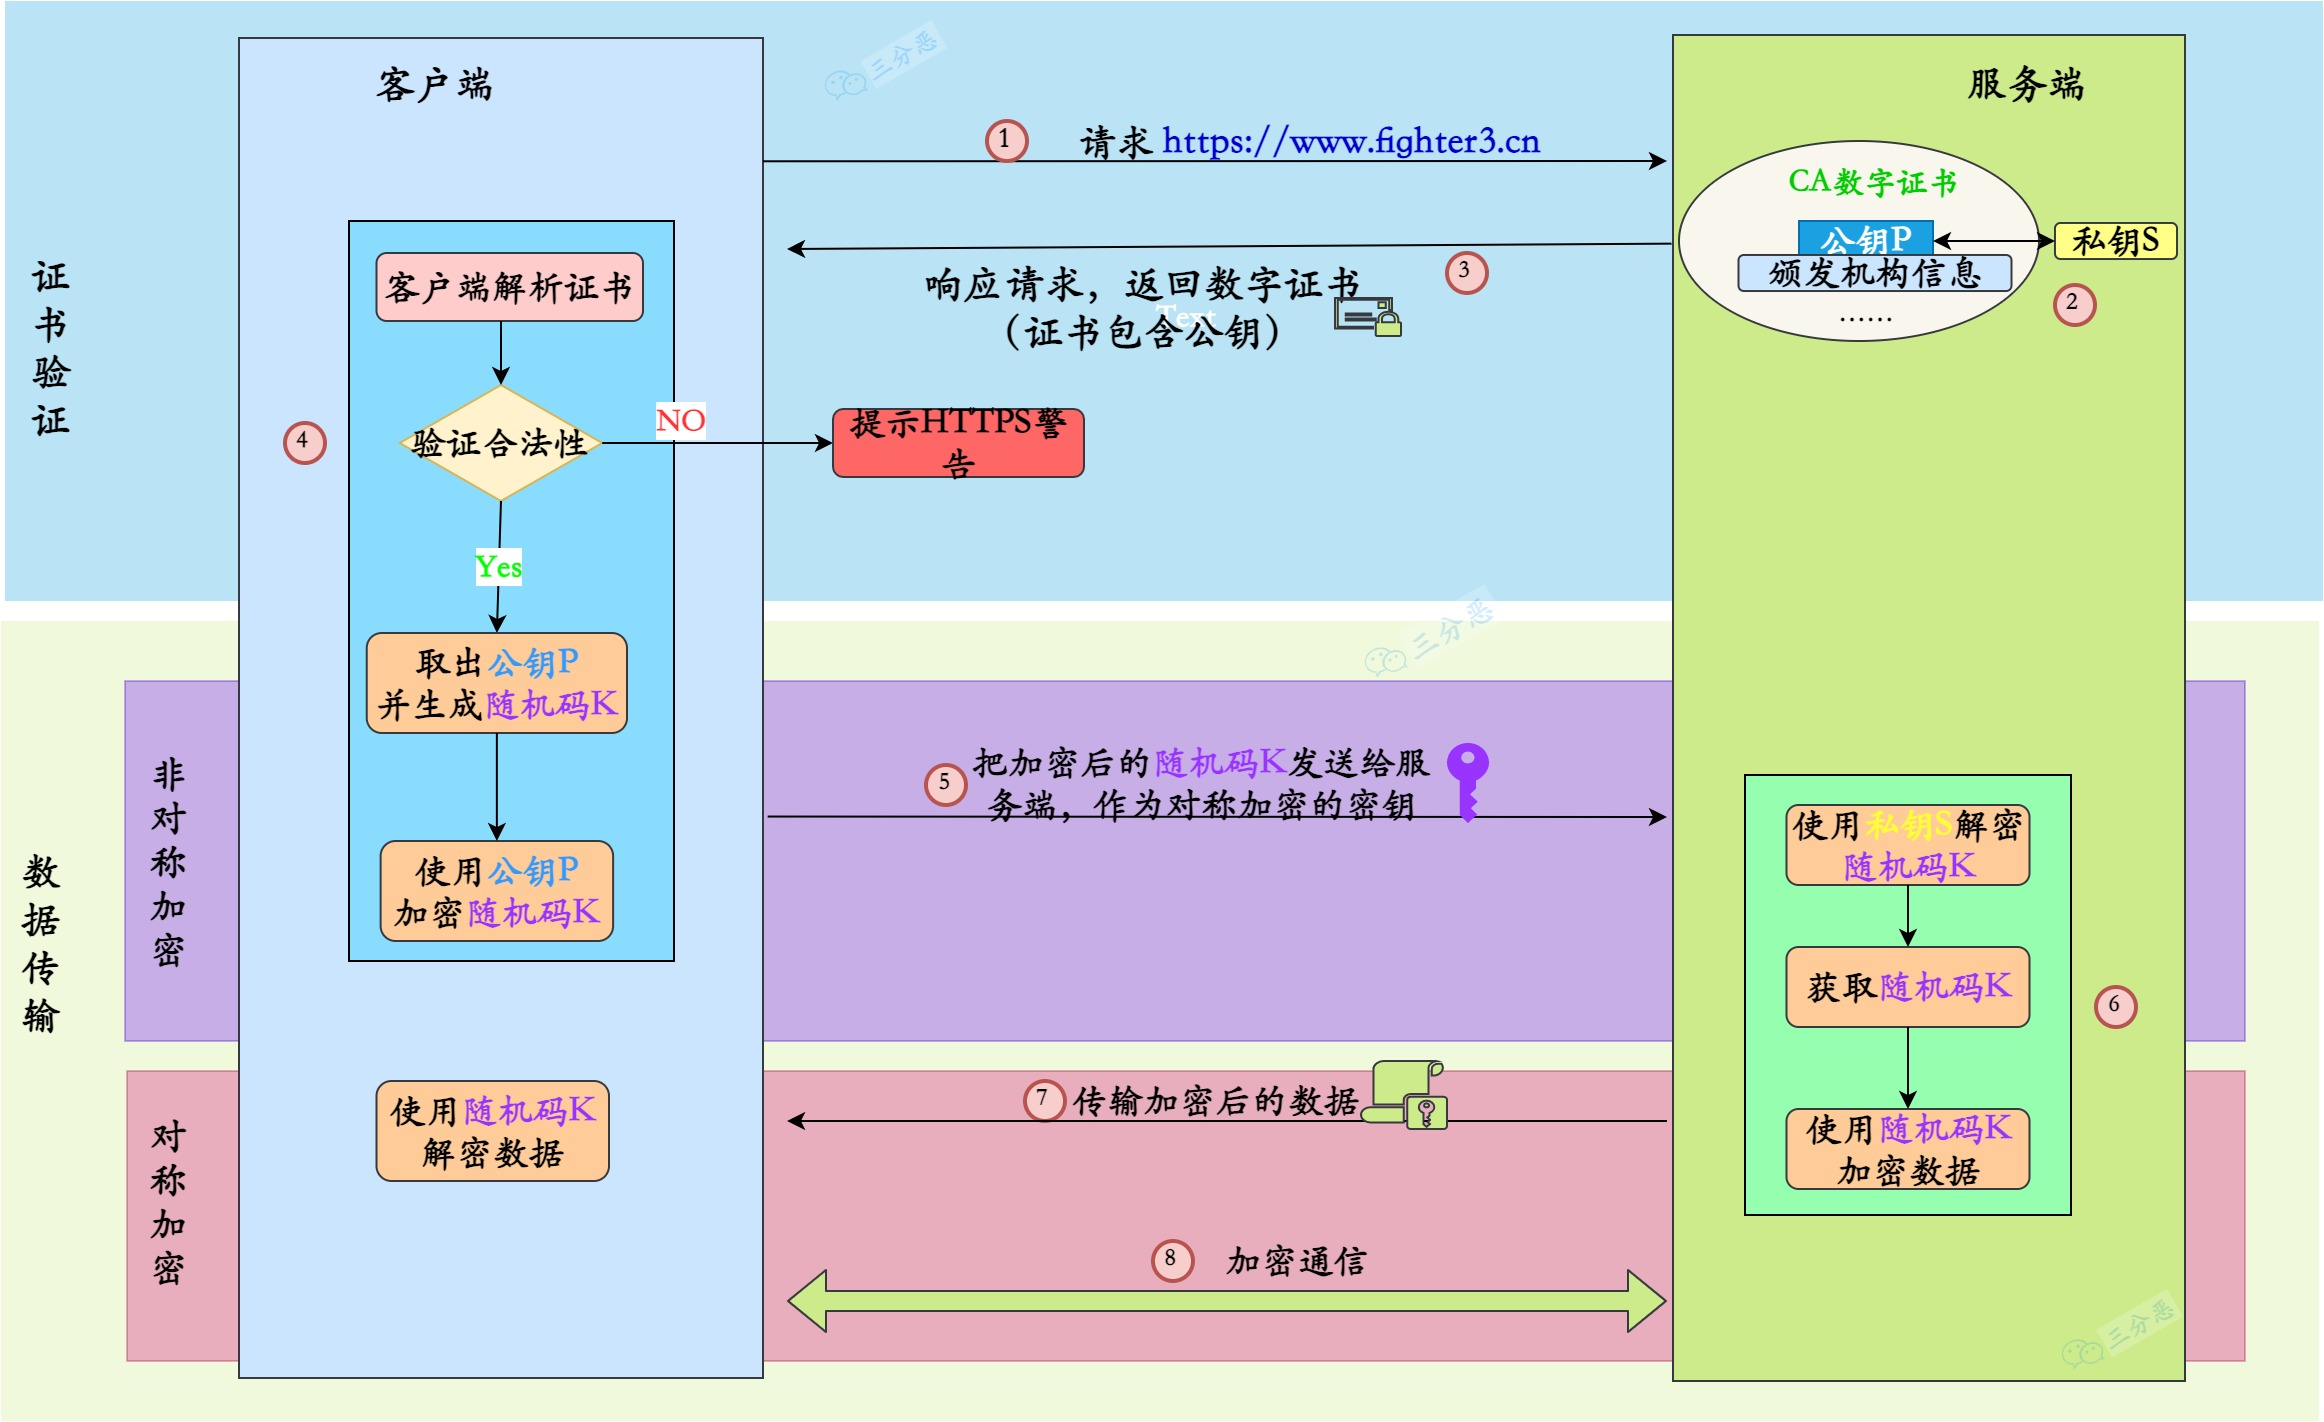
\includegraphics[width=0.7\textwidth]{./Chapter3/q26_2.png}
\caption{详细的 HTTPS 流程}
\label{fig26_2}
\end{figure}

\end{solution}

%------------- 问题27 -------------------
\begin{custom}{问题27}
客户端怎么去校验证书的合法性?
\end{custom}

\begin{solution}
首先,服务端的证书从哪来的呢?

为了让服务端的公钥被⼤家信任,服务端的证书都是由 CA (Certificate Authority,证书认证机构)签名的,CA就是⽹络世界⾥的公安局、公证中⼼,具有极⾼的可信度,所以由它来给各个公钥签名,信任的⼀⽅签发的证书,那必然证书也是被信任的。

\begin{figure}[htbp]
\centering
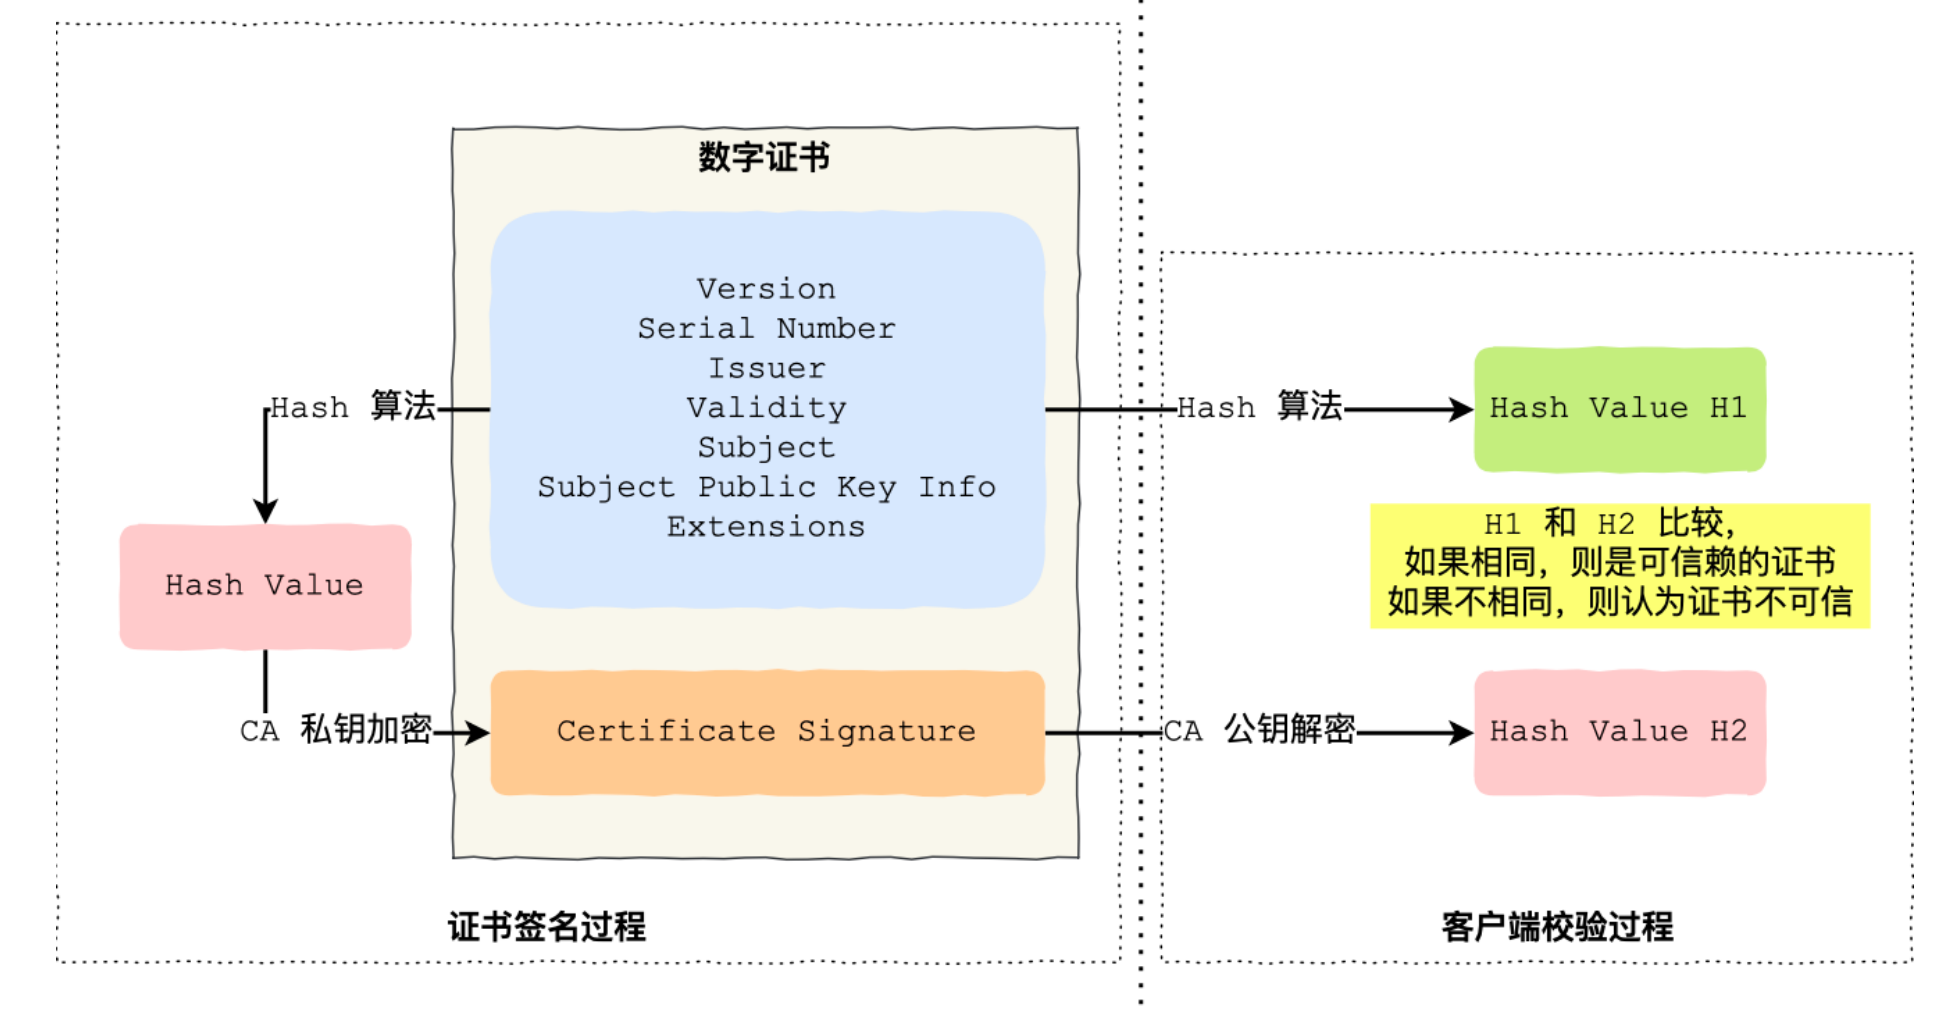
\includegraphics[width=0.7\textwidth]{./Chapter3/q27_1.png}
\caption{证书签名过程和客户端校验过程}
\label{fig27_1}
\end{figure}

CA 签发证书的过程,如上图\ref{fig27_1} 左边部分:
\begin{enumerate}
	\item ⾸先 CA 会把持有者的公钥、⽤途、颁发者、有效时间等信息打成⼀个包,然后对这些信息进⾏ Hash 计算,得到⼀个 Hash 值;
	\item 然后 CA 会使⽤⾃⼰的私钥将该 Hash 值加密,⽣成 Certificate Signature,也就是 CA 对证书做了签名;
	\item 最后将 Certificate Signature 添加在⽂件证书上,形成数字证书;
\end{enumerate}

客户端校验服务端的数字证书的过程,如上图\ref{fig27_1} 右边部分:
\begin{enumerate}
	\item ⾸先客户端会使⽤同样的 Hash 算法获取该证书的 Hash 值 H1;
	\item 通常浏览器和操作系统中集成了 CA 的公钥信息,浏览器收到证书后可以使⽤ CA 的公钥解密 Certificate
	\item Signature 内容,得到⼀个 Hash 值 H2 ;
	\item 最后⽐较 H1 和 H2,如果值相同,则为可信赖的证书,否则则认为证书不可信。
\end{enumerate}
假如在 HTTPS 的通信过程中,中间人篡改了证书原文,由于他没有 CA 机构的私钥,所以 CA 公钥解密的内容就不一致。

\end{solution}


%------------- 问题28 -------------------
\begin{custom}{问题28}
如何理解 HTTP 协议是无状态的?
\end{custom}
\begin{solution}
这个无状态的的状态值的是什么?是客户端的状态,所以字面意思,就是HTTP协议中服务端不会保存客户端的任何信息。

比如当浏览器第一次发送请求给服务器时,服务器响应了;如果同个浏览器发起第二次请求给服务器时,它还是会响应,但是呢,服务器不知道你就是刚才的那个浏览器。

那有什么办法记录状态呢?

主要有两个办法,Session 和 Cookie。
\end{solution}

%------------- 问题29 -------------------
\begin{custom}{问题29}
说说Session 和 Cookie 有什么联系和区别?
\end{custom}
\begin{solution}
先来看看什么是 Session 和 Cookie :

\begin{itemize}
	\item Cookie 是保存在客户端的一小块文本串的数据。客户端向服务器发起请求时,服务端会向客户端发送一个 Cookie,客户端就把 Cookie 保存起来。在客户端下次向同一服务器再发起请求时,Cookie 被携带发送到服务器。服务端可以根据这个 Cookie 判断用户的身份和状态。
	\item Session 指的就是服务器和客户端一次会话的过程。它是另一种记录客户状态的机制。不同的是cookie 保存在客户端浏览器中,而 session 保存在服务器上。客户端浏览器访问服务器的时候,服务器把客户端信息以某种形式记录在服务器上,这就是 session。客户端浏览器再次访问时只需要从该 session 中查找用户的状态。
\end{itemize}

\begin{figure}[htbp]
\centering
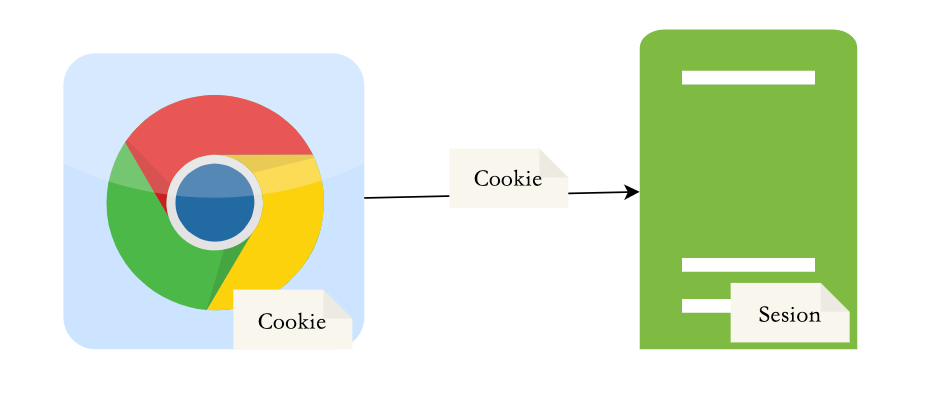
\includegraphics[width=0.7\textwidth]{./Chapter3/q29_1.png}
\caption{cookie 和 session}
\label{fig29_1}
\end{figure}

\begin{note} \textbf{Session 和 Cookie 到底有什么不同呢?} \end{note}
\begin{itemize}
	\item 存储位置不一样,Cookie 保存在客户端,Session 保存在服务器端。
	\item 存储数据类型不一样,Cookie 只能保存ASCII,Session可以存任意数据类型,一般情况下我们可以在 Session 中保持一些常用变量信息,比如说 UserId 等。
	\item 有效期不同,Cookie 可设置为长时间保持,比如我们经常使用的默认登录功能,Session 一般有效时间较短,客户端关闭或者 Session 超时都会失效。
	\item 隐私策略不同,Cookie 存储在客户端,比较容易遭到不法获取,早期有人将用户的登录名和密码存储在 Cookie 中导致信息被窃取;Session 存储在服务端,安全性相对 Cookie 要好一些。
	\item 存储大小不同, 单个 Cookie 保存的数据不能超过 4K,Session可存储数据远高于 Cookie。
\end{itemize}

\begin{note} \textbf{Session 和 Cookie 有什么关联呢?} \end{note}
\begin{figure}[htbp]
\centering
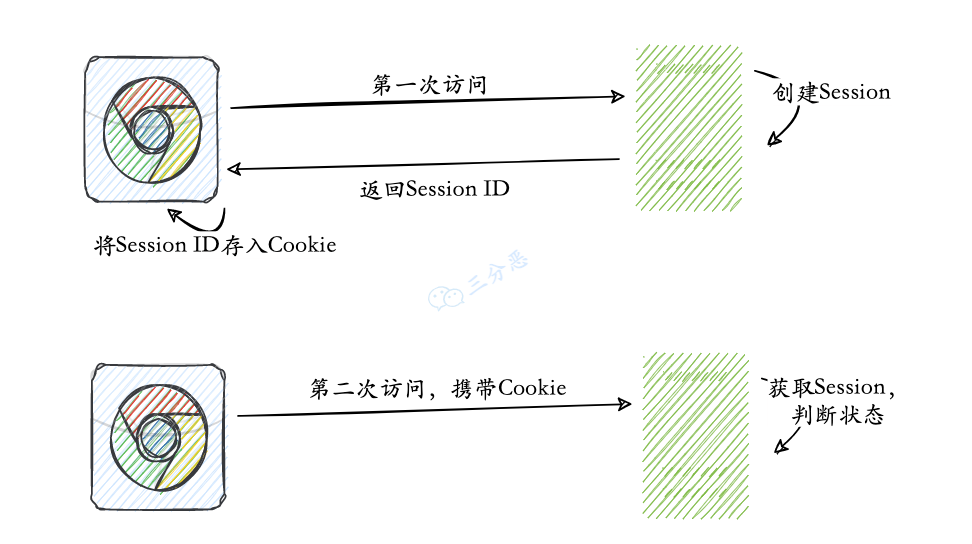
\includegraphics[width=0.7\textwidth]{./Chapter3/q29_2.png}
\caption{cookie 和 session 的创建}
\label{fig29_2}
\end{figure}
\begin{itemize}
	\item 用户第一次请求服务器时,服务器根据用户提交的信息,创建对应的 Session,请求返回时将此 Session 的唯一标识信息 SessionID 返回给浏览器,浏览器接收到服务器返回的 SessionID 信息后,会将此信息存入 Cookie 中,同时 Cookie 记录此 SessionID 是属于哪个域名。
	\item 当用户第二次访问服务器时,请求会自动判断此域名下是否存在 Cookie 信息,如果存在,则自动将 Cookie 信息也发送给服务端,服务端会从 Cookie 中获取 SessionID,再根据 SessionID 查找对应的 Session 信息,如果没有找到,说明用户没有登录或者登录失效,如果找到 Session 证明用户已经登录可执行后面操作。
\end{itemize}

\begin{note} \textbf{分布式环境下Session怎么处理呢?} \end{note}

分布式环境下,客户端请求经过负载均衡,可能会分配到不同的服务器上,假如一个用户的请求两次没有落到同一台服务器上,那么在新的服务器上就没有记录用户状态的 Session。

这时候怎么办呢?

可以使用 Redis 等分布式缓存来存储 Session,在多台服务器之间共享。
\begin{figure}[htbp]
\centering
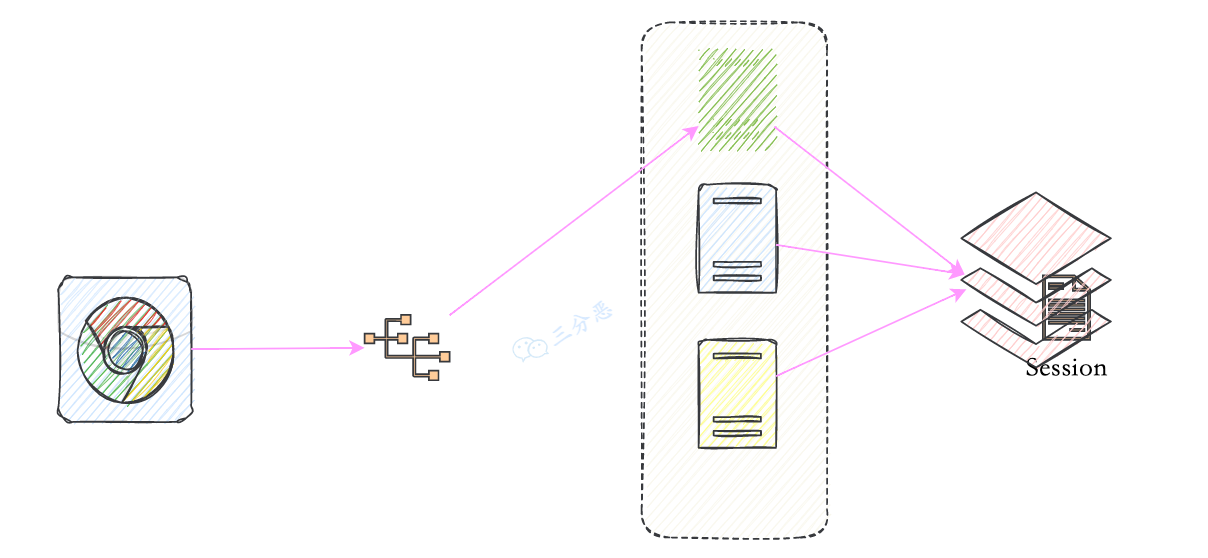
\includegraphics[width=0.5\textwidth]{./Chapter3/q29_3.png}
\caption{Redis 分布时存储 Session}
\label{fig29_3}
\end{figure}

\begin{note} \textbf{客户端无法使用Cookie怎么办?} \end{note}

有可能客户端无法使用 Cookie,比如浏览器禁用 Cookie,或者客户端是安卓、IOS 等等。

这时候怎么办?SessionID 怎么存?怎么传给服务端呢?

首先是 SessionID 的存储,可以使用客户端的本地存储,比如浏览器的 sessionStorage。

接下来怎么传呢?
\begin{itemize}
	\item 拼接到 URL 里:直接把 SessionID 作为 URL 的请求参数
	\item 放到请求头里:把 SessionID 放到请求的 Header 里,比较常用。
\end{itemize}

\end{solution}


\chapter{传输层对应问题}

%------------- 问题30 -------------------
\begin{custom}{问题30}
TCP是如何实现差错控制的?
\end{custom}
\begin{solution}
xxxxxxxxxxxxxxxxxxxx
\end{solution}

%------------- 问题31 -------------------
\begin{custom}{问题31}
详细说一下 TCP 的三次握手机制
\end{custom}
\begin{solution}
PS:TCP三次握手是最重要的知识点,一定要熟悉到问到即送分。

TCP 提供面向连接的服务,在传送数据前必须建立连接,TCP 连接是通过三次握手建立的。其过程如下图\ref{fig31_1} 所示:
\begin{figure}[htbp]
\centering
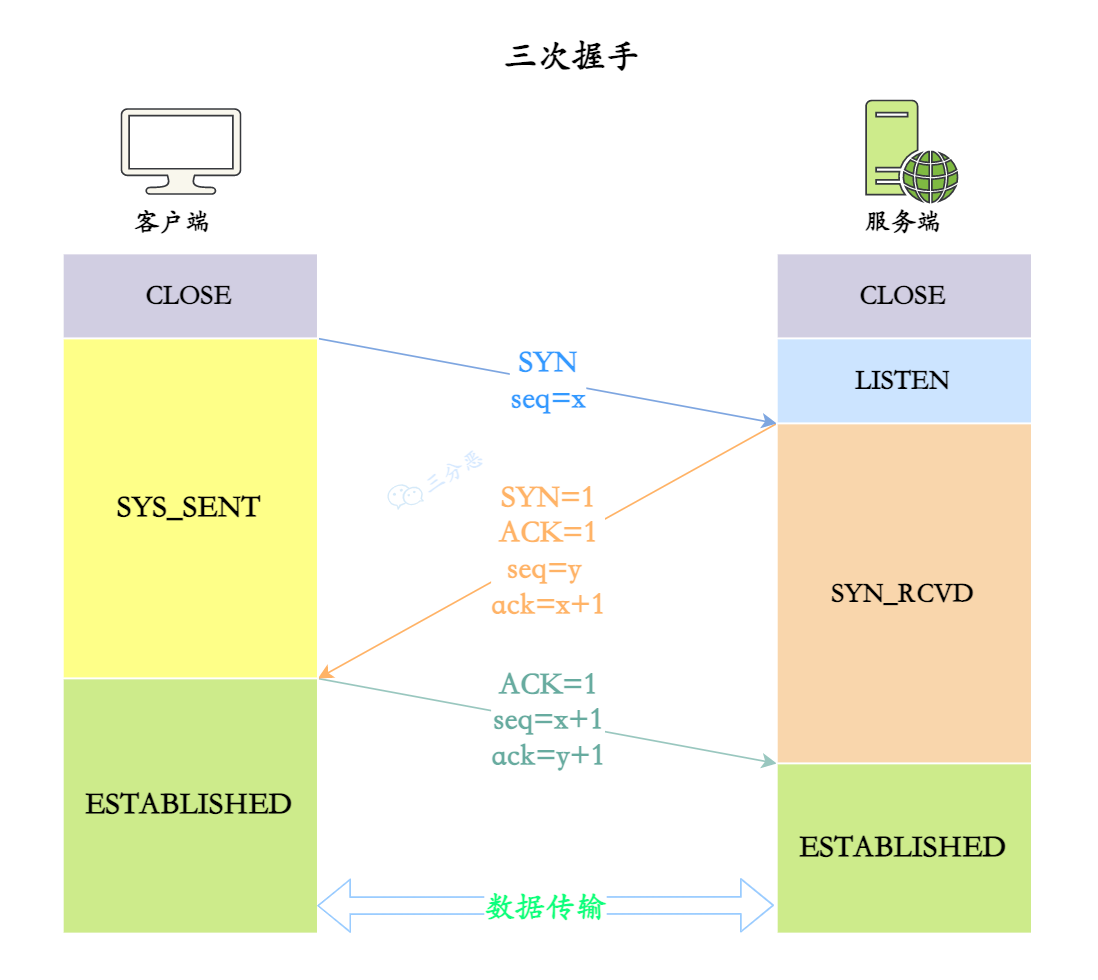
\includegraphics[width=0.7\textwidth]{./Chapter4/q31_1.png}
\caption{TCP 三次握手连接}
\label{fig31_1}
\end{figure}

三次握手的过程:
\begin{enumerate}
	\item 最开始,客户端和服务端都处于 CLOSE 状态,服务端监听客户端的请求,进入 LISTEN 状态
	\item 客户端端发送连接请求,\textbf{第一次握手}(SYN=1, seq=x),发送完毕后,客户端就进入 SYN\_SENT 状态
	\item 服务端确认连接,\textbf{第二次握手}(SYN=1, ACK=1, seq=y, ACKnum=x+1), 发送完毕后,服务器端就进入 SYN\_RCV 状态。
	\item 客户端收到服务端的确认之后,再次向服务端确认,这就是\textbf{第三次握手} (ACK=1,ACKnum=y+1),发送完毕后,客户端进入 ESTABLISHED 状态,当服务器端接收到这个包时,也进入 ESTABLISHED 状态。
\end{enumerate}

TCP三次握手通俗比喻:在二十年前的农村,电话没有普及,手机就更不用说了,所以,通信基本靠吼。老张和老王是邻居,这天老张下地了,结果家里有事,热心的邻居老王赶紧跑到村口,开始叫唤老王。

\begin{enumerate}
	\item 老王:老张唉!我是老王,你能听到吗?
	\item 老张一听,是老王的声音:老王老王,我是老张,我能听到,你能听到吗?
	\item 老王一听,嗯,没错,是老张:老张,我听到了,我有事要跟你说。"你老婆要生了,赶紧回家吧!"
\end{enumerate}  

老张风风火火地赶回家,老婆顺利地生了个带把的大胖小子。握手的故事充满了幸福和美满。
\begin{figure}[htbp]
\centering
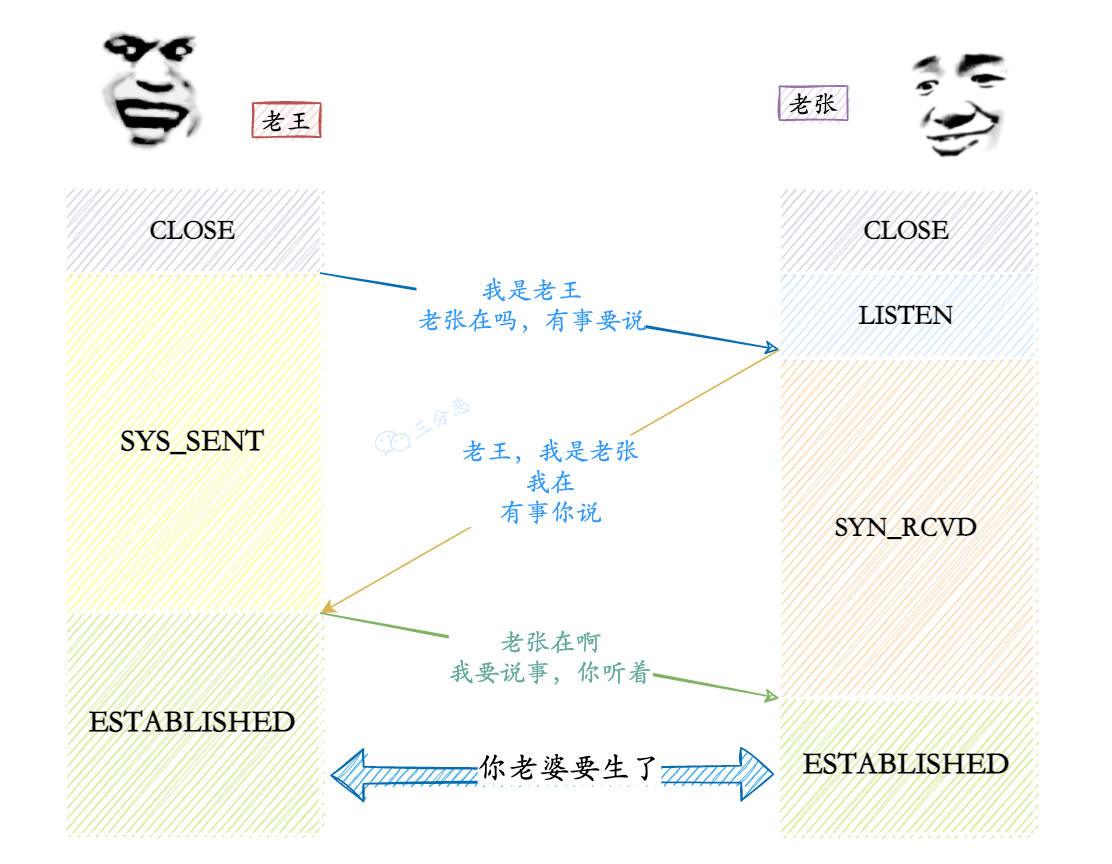
\includegraphics[width=0.7\textwidth]{./Chapter4/q31_2.png}
\caption{三次连接通话}
\label{fig31_2}
\end{figure}
\end{solution}

\end{document}
